% Nejprve uvedeme tridu dokumentu s volbami
\documentclass[czech,bachelor]{diploma}
% Dalsi doplnujici baliky maker
\usepackage[autostyle=true,czech=quotes]{csquotes} % korektni sazba uvozovek, podpora pro balik biblatex
\usepackage[backend=biber, style=iso-numeric, alldates=iso]{biblatex} % bibliografie
\usepackage{dcolumn} % sloupce tabulky s ciselnymi hodnotami
\usepackage{subfig} % makra pro "podobrazky" a "podtabulky"
\usepackage[cpp]{diplomalst}
\usepackage{pgf-pie}
\usepackage{pgfplots}
% \usepackage{pdfpages}
% \usepackage{svg}

% Zadame pozadovane vstupy pro generovani titulnich stran.
\ThesisAuthor{Lukáš Moravec}

\ThesisSupervisor{Ing. Radoslav Fasuga, Ph.D.}

\CzechThesisTitle{Nástroj pro automatizované generování reklamních grafických bannerů a videí}

\EnglishThesisTitle{Tools for Automated Generation of Promo Graphic Sources and Videos}

\SubmissionYear{2021}

% Pokud nechceme nikomu dekovat makro zapoznamkujeme.
\Acknowledgement{Rád bych na tomto místě poděkoval vedoucímu bakalářské práce, Ing.~Radoslavovi~Fasugovi,~Ph.D., za věnovaný čas, vstřícnost a ochotu ke konzultacím při vytváření této práce. Dále bych chtěl také poděkovat své přítelkyni a rodině za neustálou podporu.}

\CzechAbstract{Tato bakalářská práce je cílená na problematiku automatizovaného generování reklamních bannerů. V první části se zaměřuje na to co to vlastně reklama je, jak funguje a nejčastější způsoby toho, jak využít různé formy reklamy k dosažení svých cílů. Dále popisuje tvorbu bannerů a podmínky pro nasazení do různých reklamních sítí. Analyzuje a porovnává existující nástroje k tvorbě reklamních materiálů a jejich možnosti automatizace tvorby. Následně pojednává o tom, jak vytvořit nástroj, který by automatizaci tvorby bannerů umožňoval. Popisuje důležité funkce úprav nezbytné k efektivnímu vytváření reklamních materiálů. Výsledná aplikace je jednostránková webová aplikace, sestavená za pomoci frameworku Angular a knihovny Konva.js.}

\CzechKeywords{Reklama; Banner; Online grafika; Angular; Konva.js; SPA}

\EnglishAbstract{This bachelor's thesis is aimed at the problematics of automated generation of advertising banners. In first part, the thesis focuses on what an advertisement really is, how it works and the most common ways of how to use different forms of advertising to achieve it's goals. It also describes the creation of banners and conditions for deployment in advertising networks. It analyses and compares existing tools to create advertising materials and their options of automated creation. It then discusses on how to create a tool, which would enable automated creation of banners. The thesis describes important editing features necessary to effective creation of advertising materials. The final application is a single page web application build with Angular framework and Konva.js library}

\EnglishKeywords{Advertisement; Banner; Online graphics; Angular; Konva.js; SPA}

% \AddAcronym{DVD}{Digital Versatile Disc}
% \AddAcronym{TNT}{Trinitrotoluen}
% \AddAcronym{UML}{Unified Modeling Language}
% \AddAcronym{HTML}{Hyper Text Markup Language}
% \AddAcronym{TUG}{\TeX{} Users Group}

\addbibresource{bibliography.bib}

% Novy druh tabulkoveho sloupce, ve kterem jsou cisla zarovnana podle desetinne carky
\newcolumntype{d}[1]{D{,}{,}{#1}}

% Zacatek dokumentu
\begin{document}

% Nechame vysazet titulni strany.
\MakeTitlePages

% A nasleduje text zaverecne prace.
\chapter{Úvod}
\label{chap:Introduction}
Internetová reklama se rychle rozšířila a v momentální době se stala jednou z nejpoužívanějších. Každoroční investice do v miliardách korun jen dále podporují tento fakt.
Nejvíce viditelná grafická reklama se vyskytuje převážně ve formě bannerů a videí. Ty musí být vytvořeny ve více rozměrech, aby byly dobře viditelné na různých zařízeních.
V případě prodeje širokého množství produktů, se tvorba takových bannerů stává časově náročná. Zároveň se zde nabízí možnost automatizace tohoto procesu, díky které by se 
časové měřítko tvorby reklamního materiálu smrsklo o velkou část.
Tato práce v první cílí na objasnění toho, co to vlastně reklama je z hlediska součástí marketingu organizace. V návaznosti na to rozebírá různé formy reklamy, jejich efektivitu
a nosiče. Detailněji jsou zde popsány možnosti nasazení reklamy do Internetového prostředí společně s tím, jak monitorovat zda si inzerce vede dobře nebo špatně.
Následně se práce zaměřuje na problematiku tvorby reklamních bannerů a nasazení do reklamních sítí jako je např. Google nebo Facebook.

Druhá část je zaměřena na analýzu aktuálních nástrojů pro tvorbu grafických promo materiálů. Prozkoumává jejich možnosti automatizace, úprav, animací, technologické zpracování a možnosti
přímého napojení do reklamních sítí.
Ná základě této analýzy vzniká návrh vlastního řešení. V této části jsou vypsány potřebné možnosti úprav, které by měla výsledná aplikace poskytovat. Podle daných potřeb
se vybírají technologie umožňující tyto vlastnosti co nejjednodušejí a nejlépe implementovat. Nejdůležitější funkce nástroje jsou rozebrány více do hloubky společně s možnostmi,
jak projekt ukládat.
V neposlední řadě práce popisuje vytvořenou aplikaci a způsob, jakým aplikace funguje.


\endinput
\chapter{Teoretická část}
\label{chap:theoretical}
Reklamy se staly součástí životů většiny populace. Působí na lidskou mysl, přestože si to lidé nemusí ani uvědomovat.
Nasycené trhy dávají pro začínající podnikatele malou šanci úspěchu. Aby se mohli prosadit, musí nejen přinést světu jedinečný výrobek/službu,
ale také umět svůj produkt dobře reprezentovat a prosadit jej. Pro obchodníky se zavedenou tradicí a pozicí na trhu je zase nutné,
aby byly schopni své zákazníky udržet a nalákat nové. Pokud firma disponuje širokou nabídkou zboží,
vytváření grafické reklamy se stává časově náročnější.
Účelem této práce je prozkoumat možnosti automatizace jak tvorby, tak nasazení reklamy. 

V této kapitole jsou popsány základní pojmy týkající se marketingu a reklamy. Ve stručnosti jsou také popsány různé možnosti šíření reklamy
a srovnání jejich využitelnosti.

\section{Marketing}
\label{sec:marketing}
Účelem marketingu je poznávání, předvídání, ovlivňování a uspokojování potřeb a přání zákazníka způsobem, který je efektivní, výhodný a zajišťuje splnění
cílů firmy. Marketing vychází z trhu. Průzkum poptávky hraje důležitou roli v jeho efektivnosti.
Firma musí znát nejen momentální poptávku, ale také ji předvídat či přetvářet.

    \subsection{Marketingový mix}\label{ssec:marketing-mix}
    Marketingový mix je označení souhrnu základních nástrojů, které marketing využívá k dosažení cílů firmy.
    Existuje více alternativ tohoto mixu vycházejících z rozdílných pohledů na problém.
    Pohled ze strany podniku je označován jako 4P (z angl. Product, Price, Place, Promotion),
    zatímco z pohledu zákazníka se jedná o 4C (z angl. Customer value, Cost, Communication, Convenience).
    Tato práce se dále zabývá podnikovým mixem, konkrétně problému propagace.

    \subsection{Marketingová propagace}\label{ssec:marketing-propagation}
    \begin{quote}
        \enquote{\emph{Společenská praxe definuje pojem propagace jako uvedení něčeho nebo někoho v obecnou známost.
        Propagace v marketingovém pojetí je uvědomělá činnost, která informuje, přesvědčuje a ovlivňuje nákupní chování zákazníka.}}
        (SVĚTLÍK, J., 2016) \cite{svetlik:marketing}
    \end{quote}

    Marketingová propagace je součástí komunikačního mixu, který zahrnuje:
        \begin{itemize}
            \item podporu prodeje,
            \item reklamu,
            \item vztahy s veřejností,
            \item osobní prodej,
            \item přímý marketing.
        \end{itemize}
    Optimální strategii pro budování cíle komunikace zachycuje tzv. AIDA model. Ten zahrnuje tyto 4 kroky:
        \begin{enumerate}
            \item Získání pozornosti zákazníka.
            \item Vzbuzení zájmu.
            \item Vyvolat touhu po službě nebo produktu.
            \item Akce zákazníka.
        \end{enumerate}
    S propagací se úzce pojí \emph{cesta zákazníka}, která modeluje chování možných zákazníků na základě jejich vlastností,
    věku, osobností, trendů atd. Tento nástroj dokáže být velice užitečný v budování komunikační strategie tzn. reklamní slogany,
    cílovou skupinu, média pro šíření reklamy apod. 

    Pro efektivní propagaci je důležité, aby byla odrazem firemní identity. Firemní identita určuje způsob, jakým se firma prezentuje
    a to nejen vnějšímu světu ale také ve vlastních prostorách a ke svým zaměstnancům. Vizuální prvky firemní identity se obvykle doporučuje shrnout do
    jednoho dokumentu zvaný \emph{grafický manuál}.

    \subsection{Grafický manuál}\label{ssec:marketing-graphic-manual}
    Tento dokument přesně definuje vizuální elementy, kterými se firmy identifikují na otevřeném trhu.
    Součástí může být logo firmy, jeho různé barevné variace včetně návodů, jak je správně používat. V grafickém manuálu se specifikují textové fonty.
    Osvědčeným postupem je vybrat více fontů z důvodu dostupností na různých platformách. 

    Doporučuje se vybírat barvy podle standardizovaného vzorníku \emph{Pantone}. Důvodem je,
    že tyto barvy se na tištěném papíře velice podobat digitálním kopiím. Tiskárny a jejich subtraktivní barevný model CMYK totiž nedokáže přesně replikovat
    všechny barvy, které lze zobrazit počítačem. 

    Grafický manuál však může také obsahovat vzhled patičky internetové pošty, klasických papírových obálek,
    hlavičku a patičku dokumentů, ostatních tiskovin apod. 

    \section{Reklama}
    \begin{quote}
        \enquote{\emph{Ačkoliv reklama je pouze jedna z částí komunikačního (propagačního) mixu, je to část, která je nejvíce vidět.
        Mezi hlavní cíle reklamy patří kromě zvýšení poptávky a vyvolání nové či opakované koupě především tvorba silné značky,
        která zaujímá pevné a přední místo v mysli zákazníka mající k ní pozitivní postoj, dále identifikace a
        odlišení produktu (značky) od podobných produktů nabízených na trhu,
        vytváření pozitivní image firmy nebo výrobku a budování tak preferencí a věrnosti, posílení finanční pozice podniku,
        zvýšení možnosti distribuce a snížení nákladů spojených s prodejem, ale i motivace vlastních pracovníků aj.}}
        (SVĚTLÍK, J., 2016) \cite{svetlik:marketing}
    \end{quote}
    

    Síla reklamy se skrývá i ve schopnosti ovlivňování názorů lidí. Tohoto si lze nejčastěji všimnout např.
    u politických stran. Nejčastější reklamy lze podle způsobu použití dělit na 2 kategorie. \cite{marketing:product-vs-brand}

    \subsection{Produktová reklama}
    Tento druh reklamy je zaměřený na nabízený produkt, který se snaží vyzdvihnout výhody nad konkurencí.
    Jde o konkrétní nabízené služby nebo výrobky. Vhodné využití této reklamy je následující:
    \begin{itemize}
        \item Pokud je potřeba produktem oslovit velké publikum.
        \item Pokud je produkt skutečně \enquote{něčím dosud neviděným}.
        \item Pokud produkt \enquote{dokáže mluvit za sebe}.
    \end{itemize}

    \subsection{Značková reklama}
    Oproti produktové reklamě, se zde jedná spíše o zaujetí zákazníka jako takového. Nenabízí žádný konkrétní produkt,
    snaží se dostat zákazníkovi do podvědomí. Je výhodná pokud:
    \begin{itemize}
        \item Si značka chce vybudovat unikátní postavení na trhu. 
        \item Značka má zajímavý příběh o vzniku nebo historické pozadí. 
        \item Je prioritou budovat si zákaznickou důvěru značce. 
    \end{itemize}

    \subsection{Reklamní média}
    Jak tato práce výše zmiňuje, volba reklamního média závisí na cílové skupině, kterou se snaží oslovit.
    Správná volba dokáže pozitivně ovlivnit účinnost reklamy, zatímco špatný výběr může přinést pouze finanční zátěž.
    Média nejčastěji doručují význam reklamního sdělení 3 způsoby:
    \begin{enumerate}
        \item verbálně,
        \item zvukově,
        \item obrazově.
    \end{enumerate}
    Tato část práce rozebírá nejpoužívanější reklamní nosiče a jejich výhody. \cite{typy:medii} \cite{typy:mediatypy}
    
    \subsubsection{Tisk}
    Do této skupiny patří zejména periodické publikace jako noviny a časopisy. Tiskoviny jako katalogy, ročenky a zpravodaje zde lze také zařadit.
    Výhody tisku spočívají v geografickém zaměření -- možnost celostátního zaměření nebo jen jednotlivých regionů. Komerční sdělení se dá umístit k tématicky
    vhodným sekcím nebo časopisům. Zákazník při čtení novin a časopisů stráví více času na rozdíl od televize nebo rozhlasu,
    a proto mohou být sdělení obsáhlejší a komplexnější. Poslední výhodou jsou \emph{packshoty}, neboli společné balení inzerovaného produktu s magazínem.
    
    \subsubsection{Rozhlas}
    Rádia stejně jako noviny je možno použít pro možnost zaměření, a to nejen zeměpisným ale také časovým. Často se však stává,
    že se z rádia stane pouze kulisa na pozadí a člověk jej nevnímá. Působí pouze na jeden lidský smysl -– sluch,
    což pro nabízení určitých služeb či produktů nemusí stačit.

    \subsubsection{Outdoor}
    K této skupině se řadí jako nejpoužívanější média billboardy, citylighty, bigboardy, LED plochy a ostatní venkovní velké plochy nebo nápisy včetně
    firemních štítů, plakátů, MHD atd. Tyto nosiče setrvávají na svých místech a působí na lidi dlouhodobě, občas i vícekrát za den.
    Dají se zaměřovat od celostátního působení až na malá místa jako části měst. Nevýhodou je, že velice závisí na své lokalitě, viditelnosti a
    nemohou obsahovat složitá sdělení. 

    \subsubsection{Televize}
    Audiovizuální prezentace přes televize je jeden z nejúčinnějších prostředků komunikací s možným koncovým zákazníkem.
    Má široký rozsah uživatelů, dokáže nejlépe vyvolat emoce a asociace se značkou. Reklama se dá lépe cílit na základě měření sledovanosti.
    Její cena je však vysoká a je zde možnost, že si uživatel televize přepne kanál, aby nemusel reklamu sledovat.
    Navíc televizní inzerce se musí plánovat s předstihem z důvodů nepružných vysílacích plánů.
    
    \subsubsection{Kino}
    Ačkoli se tento typ média zdá nenápadným, má vysokou sledovanost. Divák je pohodlně usazen a v očekávání filmu věnuje svou pozornost všemu na promítacím plátně před sebou.
    Navíc je vše v perfektní kvalitě, jak zvukové, tak vizuální. Důležitým aspektem je vybrat kina s vysokou návštěvností a naplánovat reklamní kampaň předem, ideálně vložit spoty před promítání úspěšných projekcí.

    \subsubsection{Online}
    Internet je nejflexibilnější reklamní médium. Využívá jej velká část populace a rychle se rozrůstá. Nabízí různé možnosti inzercí, formátů,
    vysokou přesnost zaměření a jednoduchý monitoring. Jako jediný z výše zmíněných umožňuje interaktivní reklamu. Nabízí dobrou kontrolu nákladů a konverzí.
    Tři nejčastější způsoby platby jsou:
    \begin{itemize}
        \item PPV -- platba za zobrazení.
        \item PPA -- platba za nějakou akci (přihlášení k newsletteru, prodej, \ldots).
        \item PPC -- platba za proklik.
    \end{itemize}
    Internet přitáhl spoustu inzerentů a každý chce být co nejvíce viděn. Tímto vznikla vysoká konkurence mezi inzerenty, kdo zaplatí nejvíce za zobrazení své reklamy.
    Velký počet reklam na webu zase zapříčinil, že běžní uživatelé se chtějí reklamě vyhnout a snaží se jí blokovat.
    
    \subsubsection{Srovnání reklamních médií}
    Průzkum inzertních výkonů SPIR 2020 odhaluje, že i přes velké možnosti Internetu, je v České republice stále nejvíce investováno do reklamy televizní.
    Celkové srovnání medií se nachází na obrázku \ref{fig:spir-mediatypes}.


    \begin{figure}[h]
        \centering
        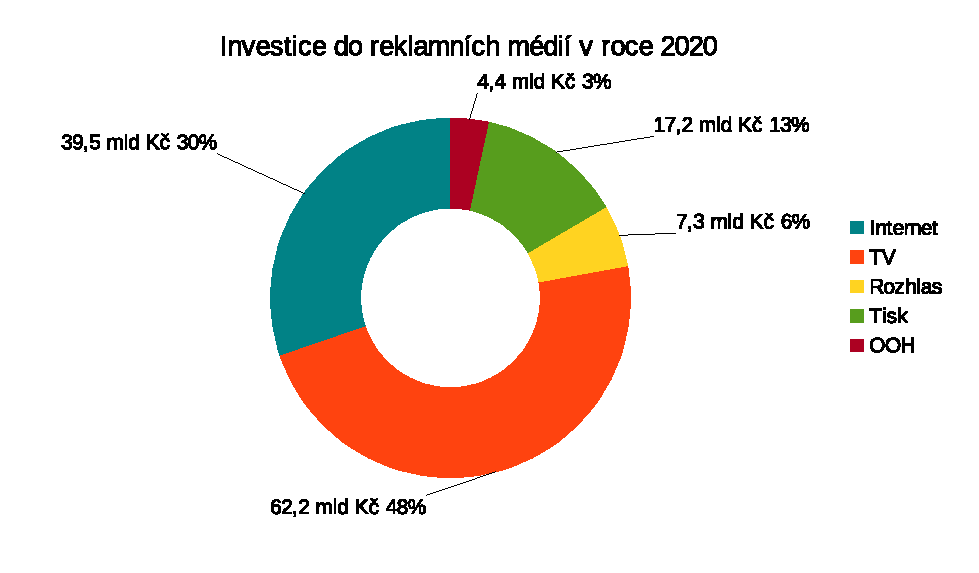
\includegraphics[width=0.9\textwidth]{Figures/pie-chart.eps}
        \iffalse
        This is my multi-line comment
        % \includesvg{Figures/pie-chart}
        % \begin{tikzpicture}
        %     \pie[
        %         text=pin,
        %         after number=~mld.,
        %         sum=auto,
        %     ]{39.5/Internet,
        %     62.2/TV,
        %     4.4/OOH,
        %     17.2/Tisk,
        %     7.3/Rozhlas}
        % \end{tikzpicture}
        \fi

        \caption[Podíl mediatypů v roce 2020]{Podíl jednotlivých mediatypů v roce 2020 \cite{spir:mediatypes}}
        \label{fig:spir-mediatypes}
    \end{figure}

    Možnosti online reklamy jsou velice rozsáhlé a stále se vyvíjejí. Následující kapitola se více zaměřuje na možnosti Internetové inzerce.

    \section{Internetová reklama}\label{sec:online-ad}
Moderní digitální doba nabízí mnoho způsobů, kterými lze komerční sdělení šířit. Jako jedny z hlavních forem se stává grafická (display) reklama,
reklama ve vyhledávání a emailová reklama. Nejčastějšími poskytovateli se stali sociální sítě a vyhledávače.
Obrovské množství denních uživatelů z nich udělali perfektní platformy pro nabízení inzercí.
Obrázek \ref{fig:spir-publishers} a tabulka \ref{tab:spir-publishers} zobrazují srovnání návštěvnosti 5 největších poskytovatelů online reklamy v České republice.

\begin{figure}[h]
    \centering
    \caption[Graf návštěvosti provozovatelů reklamních sítí]{Graf návstěvnosti reálných uživatelů provozovatelů reklamních sítí v ČR \cite{gemius:rating}}
    \label{fig:spir-publishers}
    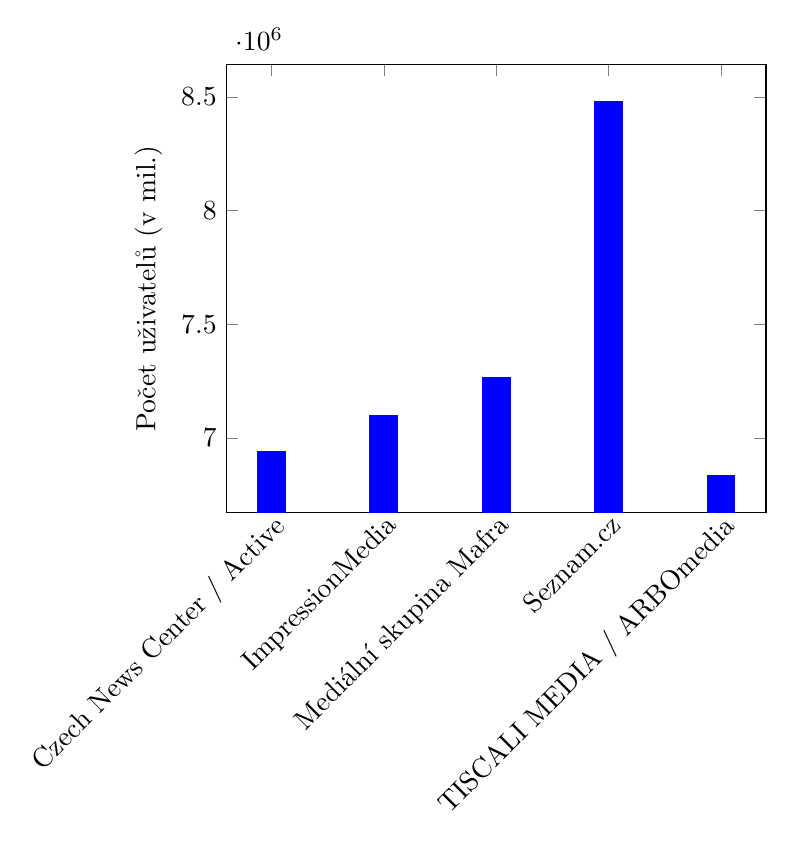
\begin{tikzpicture}
        \begin{axis}[
            symbolic x coords={Czech News Center / Active, ImpressionMedia, Mediální skupina Mafra, Seznam.cz, TISCALI MEDIA / ARBOmedia },
            x tick label style={rotate=45, anchor=north east, inner sep=0mm},
            xtick=data,
            ylabel=Počet uživatelů (v mil.),
          ]
            \addplot[ybar, fill, blue] coordinates {
                (Czech News Center / Active, 6938568)
                (ImpressionMedia,            7100320)
                (Mediální skupina Mafra,     7266377)
                (Seznam.cz,                  8480248)
                (TISCALI MEDIA / ARBOmedia,  6836590)
            };
        \end{axis}
    \end{tikzpicture}
    
\end{figure}

\begin{table}[hb]
    \centering
    \caption[Srovnání provozovatelů reklamních sítí]{Srovnání provozovatelů reklamních sítí \cite{gemius:rating}}
	\label{tab:spir-publishers}
    \begin{tabular}{l|r|r|r|r}
        \toprule
            Název & Reální uživatelé & Zobrazení stránky & Návštěvy & Čas \\
        \midrule
            Seznam.cz & 8 480 248 & 4 541 397 144  & 1 104 367 612 & 13782r 58d  \\
            Mediální skupina Mafra & 7 266 377 & 741 803 207  & 128 011 647  & 1156r 302d \\
            ImpressionMedia & 7 100 320  & 258 039 333 & 91 386 082 & 370r 7d  \\
            Czech News Center / Active & 6 938 568 & 508 776 721 & 110 070 333  & 549r 310d  \\
            TISCALI MEDIA / ARBOmedia & 6 836 590 & 120 326 836  & 44 648 445 & 204r 83d  \\
        \midrule
        
    \end{tabular}
\end{table}


Co se týče emailové reklamy, považuje se efektivní formu přímého marketingu, která je navíc zdarma.
Firmy mohou komunikovat se svými zákazníky jakožto stálými odběrateli nebo rozesílat hromadné emaily. Legislativně je však nevyžádaná elektronická pošta ošetřena.
Organizace tedy při posílaní emailů si musí být jisté, že je jejich sdělení oprávněné a nebude označeno jako spam.

Reklama ve vyhledávání se stává již placenou, většinou stylem PPC. Zadavatelé se za příplatek dostanou na první pozice výsledku hledání.
Toto jim zajišťuje vyšší míru prokliků a lépe nalákají potenciální zákazníky na svou webovou stránku. 

Grafická reklama (nejčastěji bannery a videa) je silným nástrojem pro rozšíření působnosti značky. Buduje povědomí o značce a
zároveň může lákat na produkt. Obsahuje reklamní sdělení, logo firmy a výzvu k akci (CTA) -- nejčastěji ve formě tlačítka.
Obrázek \ref{fig:spir-ad-performance} Ukazuje srovnání investic do grafické a vyhledávané reklamy.

\begin{figure}[h]
    \centering
    \caption[Výkon reklam v roce 2020]{Výkon jednotlivých forem internetové reklamy v roce 2020 \cite{spir:mediatypes}}
    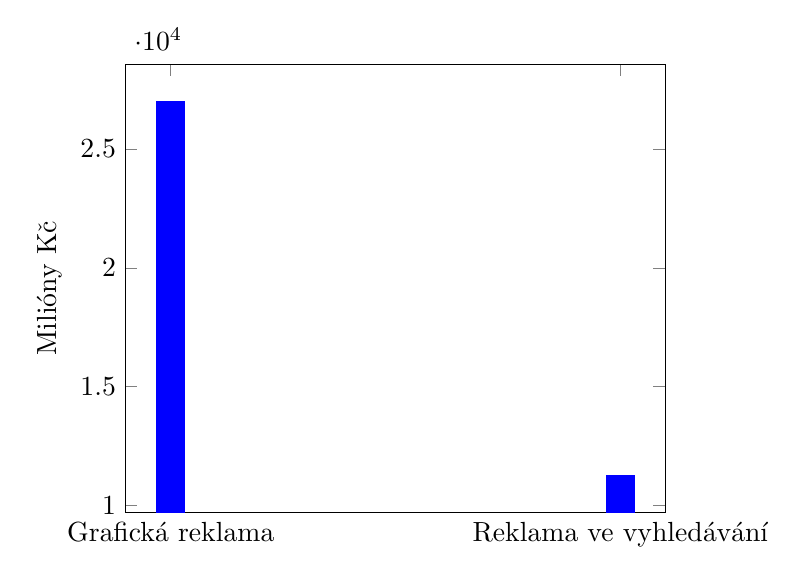
\begin{tikzpicture}
        \begin{axis}[
            symbolic x coords={Grafická reklama, Reklama ve vyhledávání},
            xtick=data,
            ylabel=Milióny Kč
          ]
            \addplot[ybar, fill, blue] coordinates {
                (Grafická reklama,           26998)
                (Reklama ve vyhledávání,     11274)
            };
        \end{axis}
    \end{tikzpicture}
    \label{fig:spir-ad-performance}
\end{figure}

    \subsection{Metriky internetových reklam}\label{ssec:online-ad-metrics}
    Jak tato práce již zmiňovala, výhodou online inzercí je jednoduchý monitoring. Na rozdíl od ostatních médií si firmy mohou být více jisté,
    že jejich reklamu cílené osoby opravdu vnímají. Hlavní metrikou reklamy vždy bývá zvýšení prodeje.
    Nicméně tato metrika se již měří obtížně a je spíše výsledkem z níže uvedených následujících ukazatelů.

        \subsubsection{Míra prokliku (CTR)}
        Takzvaná míra prokliku určuje, jak je velká šance že na reklamu někdo zareaguje kliknutím myši. Určuje se poměrem mezi celkovým počtem zobrazení reklamy a
        kliknutím na ni. Její význam spočívá v tom, že dokáže prozradit úspěšnost kampaně z hlediska upoutání pozornosti.

        \subsubsection{Míra okamžitého opuštění (BCR)}
        Tato metrika zaznamenává procento uživatelů, kteří se vlivem reklamy dostali na cílovou webovou stránku, ale neprovedou žádnou další aktivitu a
        typicky z webu odejdou. Vysoká procento BCR nejčastěji indikuje jednu z následujících věcí:
        \begin{itemize}
            \item Cílová webová stránka byla nízké kvality. Např. nezajímavý vzhled, neresponzivnost, nepřístupnost, dlouhá doba načítání atd.
            \item Produkt nebo služba nabízená v reklamě nesouvisí s tím, co člověk hledal.
            \item Osoba na stránce našla vše potřebné a další informace nepotřebuje.
        \end{itemize}

        \subsubsection{Konverzní poměr (CVR)}
        Konverzní poměr je výsledkem osob, kteří skrze reklamu dostali na webovou stránku, dokončili nějakou akci (a stali se tak zákazníky) s
        celkovým počtem zobrazení stránky. Akci, kterou mají uživatelé splnit si firma určí sama. Pro e-shopy toto může znamenat dokončení objednávky,
        pro blogy třeba přehlášení k newsletteru.

        \subsubsection{Návratnost investic (ROI)}
        Inzerování je spjato s náklady a investicí. Ve své nejjednodušší podstatě je poměr nákladů a výdělku výslednou metrikou.
        Výdělkem nemusí být pouze zisk, ale i jiný cíl, který si firma stanoví (zvýšení popularity, uživatelů atd.).

    \subsection{Zobrazení online reklamy}
    Pro dobré využití reklamy je potřebné jej umístit na dobře viditelná místa webových stránek s vysokou návštěvností.
    Těmi se stali převážně sociální sítě typu Facebook, Youtube, Twitter apod. Jelikož tito giganti vlastní i více dalších podobných stránek,
    vznikly reklamní sítě jako Google Ads. To umožnilo vznik partnerských webů, které zobrazují reklamy právě prostřednictvím těchto sítí.
    Na oplátky dostávají partnerské weby část tržby ze zobrazených reklam.

    Zmiňované reklamní sítě mají za úkol dát správnou reklamu na správný web.
    Korektní stránku lze vybrat na základě jejího celkového obsahu, klíčových slov vyhledávání spotřebitele či dokonce z analýzy způsobu prohlížení stránky.
    Inzerenti si kupují \enquote{online prostor} pro svou reklamu. 

    Druhou možností je \enquote{kupovat} si cílové publikum své reklamy, a to za pomocí technologie \emph{RTB}.
    Na začátku si inzerent při tvorbě reklamní kampaně vybere svou cílovou skupinu. Tu specifikuje pomocí různých demografických kritérií apod.
    Ve zjednodušené podobě je průběh RTB znázorněn na obrázku \ref{fig:rtb}.

    \begin{figure}[h]
        \centering
        \caption[Fungování RTB]{Zjednodušený způsob fungování RTB \cite{rtb}}
        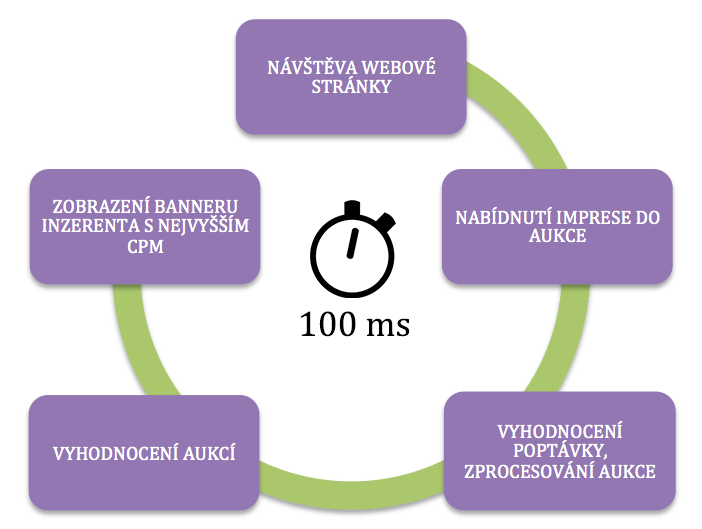
\includegraphics[width=0.7\textwidth]{Figures/rtb.png}
        \label{fig:rtb}
    \end{figure}

\endinput

    \section{Bannerová reklama}
    \begin{quote}
        \enquote{\emph{Cílem bannerové reklamy je nejen zprostředkovat reklamní sdělení, ale i zabezpečit, aby se recipient velmi jednoduchou aktivitou
        (kliknutím na banner) přesunul na požadovanou webovou lokalitu (firemní stránku, stránku značky, stránky produktu/značky na sociální síti atd.).}}
        (SVĚTLÍK, J., 2017) \cite{svetlik:reklama}
    \end{quote}

    V této části se práce více zaměřuje na bannerovou reklamu.
    Teorie a efektivita tohoto typu inzerce je zde rozebrána jako první a více do detailu. \cite{banner:advertising}

    \subsection{Formáty zobrazení}
    První webový banner se objevil na internetu v roce 1994. V té době se bannery objevovali nejčastěji jako statický obrázek ve formátu
    JPEG nebo PNG. Tento způsob zobrazení se udržel dodnes. Dynamický obsah v podobě animace bylo schopný zobrazit formát GIF a to v podobně pohyblivých obrázků.
    Společnost Macromedia s jejich technologií \emph{Flash} dokázali do bannerů přidat i možnosti interakce v podobě animací nebo přehrání zvuku při
    pohybu kurzoru myši nad bannerem. Dnes už technologie Flash z důvodu bezpečnosti a HW nároků není ve významných internetových prohlížečích podporována a
    dá se plně nahradit spojením HTML a JS kódu. 

    \subsection{Statický nebo dynamický banner}
    Statický banner je pouhým obrázkem, který se nijak nehýbe a nemá možnost interakce s uživatelem. S nástupem bannerů na Internet se u
    spotřebitelů začal objevovat fenomén zvaný \emph{bannerová slepota}. Bylo zjištěno, že někteří uživatelé podvědomě bannery na standardních místech
    úplně ignorují a nevnímají je. Proti tomuto jevu dokáži efektivně bojovat dynamické bannery.
    I krátká animace dokáže zachytit pozornost oka a tím lépe působit na cílové publikum.
    Toto se dá jednoduše změřit při porovnání CTR statických a dynamických bannerů.

    \subsection{Rozměry bannerů}
    Některé ze standardních rozměrů bannerů (v px) a jejich názvy lze vidět na obrázku \ref{fig:banner-sizes}. Podle rozlohy se zobrazují na jiných částech webových stránek nebo
    mobilních aplikací. S rozměry se také pojí velikost souborů. Reklamní sítě mívají na nahrané bannery limity velikostí.
    Čím menší velikost, tím rychleji se dokáže banner načíst. Nejčastější limit bývá 150~KB. Toto je více rozebráno v kapitole o reklamních sítích.

    \begin{figure}[h]
        \centering
        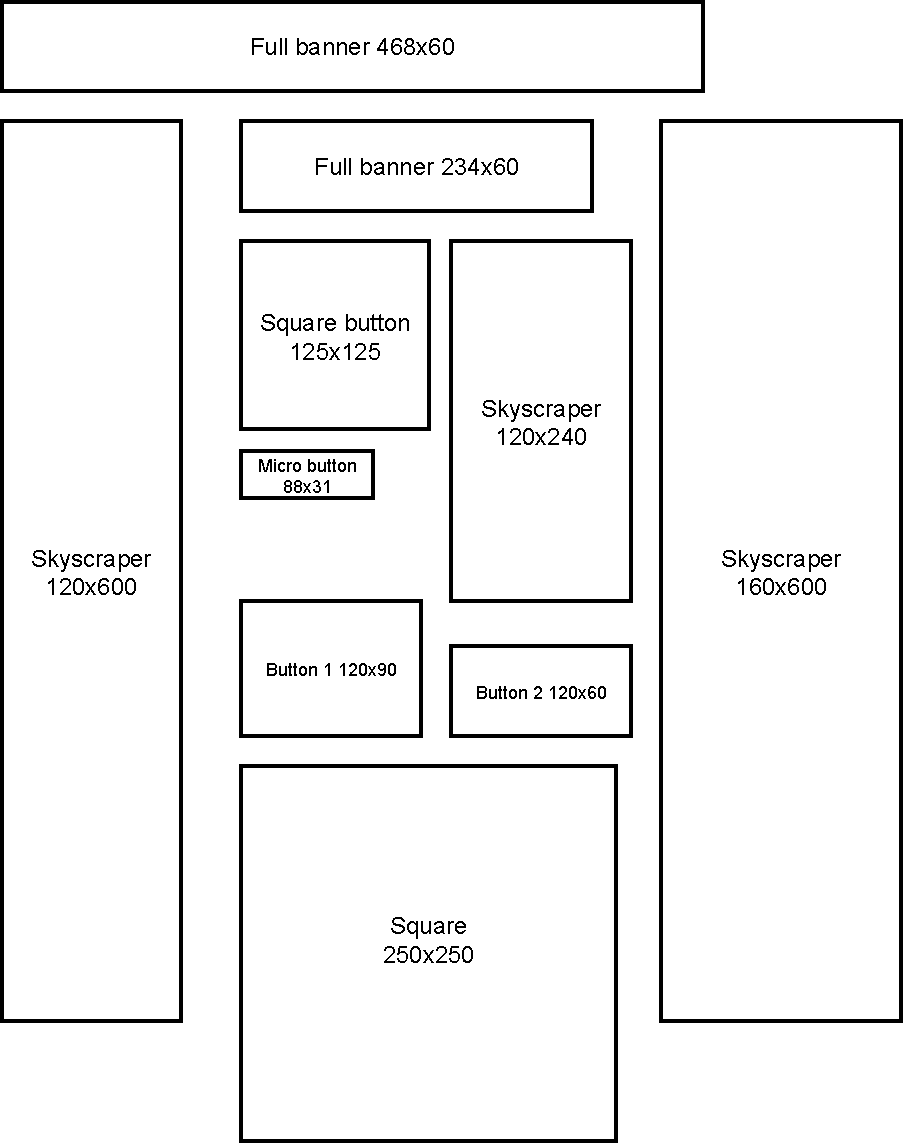
\includegraphics[width=1\textwidth]{Figures/banner-sizes.pdf}
        \caption[Velikosti bannerů]{Standardní používané velikosti bannerů}
        \label{fig:banner-sizes}
    \end{figure}

    \subsection{Jak vytvořit dobrý banner}
    Jak měřit efektivitu reklamy se zmiňuje část \ref{ssec:online-ad-metrics}. Tato část se věnuje tomu, jak banner vytvořit,
    aby již zpočátku co nejvíce upoutal zákazníky. \cite{banner:design}
    Reklamní banner se skládá ze 4 základních částí. Těmi jsou:
    \begin{itemize}
    \item logo inzerenta,
    \item titulek (komerční sdělení),
    \item pozadí,
    \item výzva k akci (CTA).
    \end{itemize}
    Na banneru se může nacházet více prvků, je však důležité, aby tyto hlavní části splnily doporučená pravidla, která jsou zde postupně rozebrána.

    \subsubsection{Logo}
    Pokud je to možné, mít logo na banneru je velice důležité. Pomáhá budovat povědomí o značce a napovídá zákazníkovi na čí webovou stránku by se měl dostat.
    Mělo by být dobře viditelné, ale nemělo by opticky přebíjet titulek nebo výzvu k akci.

    \subsubsection{Pozadí}
    Co se pozadí týče, na výběr jsou 2 varianty. Buď celobarevné nebo fotografie. Obojí má svá pro i proti. Pokud se banner snaží prodat nějaký produkt,
    je vhodnější vynechat obrázkové pozadí. Jednobarevná pozadí vytváří přirozený kontrast s výzvou k akci.
    Produkt na ni dobře vynikne a neodvádí pozornost od titulku. Naproti tomu, pokud se vytváří reklama na určitou službu nebo
    produkt nefyzického charakteru (nejčastěji software, IT služby) lze fotografií na pozadí ilustrovat onu nabízenou věc. 

    \subsubsection{Titulek}
    Doporučuje se spíše krátký text. Za úkol má přilákat pozornost možného zákazníka, tím pádem rozměrově zabírá větší část banneru.
    Podstatné kritérium je, aby byl text opět dobře čitelný. Proto je zapotřebí zvolit kontrastní barvu textu s dobře čitelným fontem.
    Řez písma by neměl být příliš tenký, jinak by text mohl splývat s pozadím nebo se špatně číst. Efekty typu zkosení se moc nedoporučují a
    někteří poskytovatelé reklamních sítí je vůbec nepovolují. 

    \subsubsection{Výzva k akci}
    Měla by u diváka vyvolat pocit nutnosti na banner kliknout. Zároveň by měla být dobře viditelná hned po titulku.
    Proto se často vyskytuje v podobě tlačítka s vhodně zvolenou barevnou kombinací.
    Umístění blíže k titulku diváka přirozeně navede.


\endinput

    \section{Poskytovatelé reklamních sítí}
\label{sec:networks}
Jak tato práce již zmiňovala, reklamám se nejlépe daří na webových stránkách s vysokou návštěvností, protože se inzerce zobrazí více návštěvníkům.
Tato část si podrobněji rozebere a porovná podmínky online bannerové reklamy od několika různých poskytovatelů. 

    \subsection{Google}
    Tento web se stal králem Internetových vyhledávačů. S průměrem kolem 3,5 miliónů vyhledávacích dotazů za minutu (celosvětově),
    jen potvrzuje své dominantní postavení. Reklamu poskytuje v rámci své služby Google Ads (dříve Google AdWords),
    která nabízí vyhledávací kampaně, obsahové kampaně a video kampaně. Co se týče bannerové reklamy,
    Google podporuje 3 formáty obrázkových souborů (PNG, JPEG, GIF) standardních specifikovaných velikostí, které řadí do 4 kategorií:
    \begin{itemize}
        \item čtvercové a obdélníkové,
        \item svislé,
        \item výsledková tabule,
        \item mobilní.
    \end{itemize}

    Lze nahrát archiv ZIP obrázků, který nesmí mít více než 40 souborů celkem a všechny obrázky musí být do max 150 KB. V případě že se jedná o GIF animaci,
    nesmí přesáhnout 30 vteřin. Zároveň v animacích nesmí být blikající efekty a frekvence snímků nesmí překročit 5 snímků za vteřinu.

    Za zmínku také stojí možnost tzv. Responzivní reklamy. Ta funguje tak, že inzerent si nahraje svá loga, produkty,
    doplní titulek a ostatní informace. Potom Google za použití strojového učení sám dynamicky sestavuje a zobrazuje kompletní bannery.
    Ovšem při tomto použití nemá inzerent plnou kontrolu nad výslednou grafikou.

    Ohledně reklamní politiku Googlu, nedovoluje propagaci padělaného zboží, nebezpečných produktů a služeb včetně tabákových výrobků,
    nevhodného a nemorálního obsahu jako např. šikana, zastrašování, vydírání, hackování, falešné dokumenty a plagiátorství. Dále, pokud osoba,
    která chce své produkty inzerovat nesmí zneužívat reklam k obsahu, který slouží pouze k navedení na koncového zákazníka někam jinam,
    shromažďovat uživatelská data k neznámým nebo nekalým účelům nebo se vydávat za někoho jiného. S určitým omezením a ohledem na zákony či věk svých koncových
    uživatelů dovoluje Google reklamy na erotický obsah, alkohol, hazardní hry, politický obsah, finanční služby, zdravotnické služby a léky.

    \subsection{Facebook}
    Facebook společně s Instagramem podporují velké množství obrázkových formátů. Ale pro nejlepší výsledky doporučují JPEG nebo PNG.
    Tento poskytovatel nezobrazuje standardní bannery, ale pouze obrázky, u kterých záleží na poměru stran.
    Velikosti a poměr stran obrázků se odvíjí podle toho, kam chceme reklamu mít umístěnou. Podporované poměry stran jsou tyto:
    \begin{itemize}
        \item 1,91:1,
        \item 16:9,
        \item 1:1,
        \item 4:5,
        \item 2:3,
        \item 9:16.
    \end{itemize}

    Každý z poměrů stran je vhodný pro zobrazení na různých místech těchto sociálních sítí (např. Kanál příspěvků, Stories, atd.).
    Kompletní tabulku je možno najít na tomto \href{https://www.facebook.com/business/help/682655495435254?id=271710926837064}{odkazu.}

    Minimální doporučené rozlišení je 1080x1080px. Oproti Googlu může být soubor velký až 30 MB.
    Reklamy na Facebooku a Instagramu musí být v souladu se zásady komunity, musí odkazovat na plně funkční úvodní stránky,
    nesmí obsahovat nezákonné produkty nebo služby, diskriminační postupy, nebezpečné doplňky stravy, tabák a s ním související produkty,
    obsah pro dospělé, dezinformace atd.

    \subsection{Sklik}
    Česká služba Sklik firmy Seznam.cz si v České republice vybudovala podobné postavení jako Google.
    Dle dat firmy Gemius, je Seznam.cz největším vydavatelem online reklamy v České republice. Pro lepší inzerci poskytuje cílení
    např. podle témat partnerských webů, zájmů uživatelů, pohlaví, klíčových slov atd.

    Povolené soubory pro nahrání bannerové reklamy jsou PNG, JPEG a GIF. Velikostně se soubory musí vlézt do max. 150 KB a
    rovněž podporuje všechny standardní velikosti bannerů.

    Bannery musí vyplňovat celou reklamní plochu, musí být jasně čitelné, relevantní, obsahově a kvalitativně srozumitelné.
    Také by měli mít textové sdělení -- krátký popis nebo výzva k akci. Reklama nesmí napodobovat, nesmí porušovat autorská práva,
    je zakázáno používat clickbaitové sdělení typu \enquote{Budete v šoku} apod. Reklama na erotický obsah se zobrazuje pouze od 22:00 do 6:00.  

\endinput




\endinput
\chapter{Analýza existujících nástrojů pro tvorbu bannerů}
\label{chap:analysis}

\section{Adobe Photoshop}
Nejznámější nástroj pro úpravy grafiky od firmy Adobe nabízí širokou škálu možností pro vytváření reklamních bannerů.
Poradí si jak se statickou grafikou tak i animovanou. Jeho profesionalita však může být pro některé uživatele náročná a nepřehledná.
Možnost převedení do HTML5 v samotném Photoshopu chybí a pro tento účel je nutné využít jiný program.

Co se týče automatizovaného generování bannerů, k Photoshopu je dostupné rozšíření zvané \emph{Banner Ad Reflow}.
To umožní uživateli definovat šablonu rozmístění objektů a pomocí umělé inteligence se pokusí optimálně obsah banneru rozmístit.
Pokud by bylo potřeba vygenerovat bannery se stejným rozložením pro více produktů, lze tohoto docílit pomocí skriptování.
To ovšem není pro všechny uživatelé vhodný přístup a velice zvyšuje celkovou složitost tvorby. Photoshop jako takový nenabízí možnost napojení na poskytovatelé reklamních sítí.

\section{Google Web Designer}
Jedná se o propracovaný desktopový designer pro tvorbu HTML5 reklamních bannerů jak statických, tak animovaných.
S řadou předpřipravených šablon na míru již daných formátů reklamy poskytovaných Googlem je tento návrhář jedním z nejsilnějších
volně dostupných produktů pro tvorbu propagačních materiálů.

Umožňuje navázat na různé prvky banneru události a jednoduše tím udělat banner více interaktivní.
Dále zahrnuje možnost práci v 3D prostoru, nebo textovém HTML editoru.
Animace lze vytvořit pouhým přetažením objektů po plátně. Upravovat jde délka animace, trasa pohybu, časovací funkce apod. 

Navíc program sám kontroluje řadu vlastností, které platforma Google Ads vyžaduje
(velikost souboru, validní HTML kód, správné URL odkazy atd.). Výslednou tvorbu je schopen přímo importovat do reklamní kampaně.

\section{Creatopy}
Tento online nástroj nabízí více svých pokročilých služeb pouze v placených verzích. Mezi jeho schopnosti však spadá vytváření HTML5 bannerů,
animací a tvorba více bannerů najednou. Poslední zmínění způsob tvorby je však limitován na pevně dané položky banneru jako logo, titulek,
tlačítko atd. Dále nabízí tvorbu Stories pro Facebook a Instagram. Na všechny možnosti poskytuje předpřipravené šablony,
které stačí upravit pro individuální potřebu.

Online editor nepoužívá pro práci element canvas, ale každý objekt je samostatný HTML element. Aplikováním kaskádových stylů je dosaženo požadovaného vzhledu.
To znamená, že možnosti úprav jsou dané možnostmi CSS, které v dnešní době sice zvládnou dostatečnou škálu efektů, jenže zavísí na podpoře prohlížečem.
Například, funkce \texttt{backdrop-filter} dokáže aplikovat různé filtry na pozadí HTML elementu, avšak zatím není v prohlížeči Firefox podporována.
Tím, že editor využívá práci přímo s HTML získává dobrou výkonnost, ale ztrácí, pokud si uživatel chce grafiku vytvořit sám.
Nástroj spoléhá spíše na využití mnoha předpřipravených tvarů, které se následně dají upravovat. Vytvořený banner umí následně zmenšit nebo
zvětšit na ostatní různé velikosti.

\section{Bannerflow}
Další prostředek tvorby bannerů prostřednictvím Internetu. Své služby nabízí v rámci předplatného.
Po zaplacení se uživatelům otevře jeden z nejpokročilejších nástrojů pro tvorbu online inzerce.
Samozřejmostí pro něj je návrh a zpracovaní grafiky. Bannery dokáže automaticky škálovat a obsah rozmístit v rámci libovolných velikostí.
Navíc oproti výše zmíněným službám umožňuje přímé napojení na hlavní poskytovatele reklamních sítí (nezmiňuje však konkrétně jaké) a
automatické nahrávání bannerů do reklamních kampaní. Dále také shromažďuje analytická data, které zpřístupňuje svým klientům přímo v rámci aplikace.

\section{Srovnání}
Ačkoli autor této práce hledal, nikde neuměl najít nástroj, který by umožnil jednoduše do stejné šablony bannerů nahrát zdroj dat textů a obrázků,
jehož výsledkem by byly bannery se stejným rozložením. Tato funkce může být vhodná například pro e-shopy,
které nabízí velké množství podobných produktů (pračky, sušičky, apod.). Pokud by tato možnost byla dostupná,
mohla by drasticky snížit celkový čas tvorby reklamy. 



\endinput
\chapter{Návrh a implementace online nástroje}
\label{chap:design}
U popisování již existujících nástrojů si lze povšimnout toho, že editory jsou svými schopnostmi pokročilé.
Dokáží efektivně pracovat s grafikou a používat různé efekty. Většinu změn lze sledovat v reálném čase. 

Online nástroj, který je součástí této práce by tedy měl mít podobnou funkcionalitu, na kterou jsou obvyklí uživatelé zvyklí.
Těmi mohou být jak zkušení grafičtí designéři, tak i lidé bez hlubší znalosti tvorby bannerů.
Rozsah této práce nepokrývá vytváření grafiky přímo v editoru, a proto bude nástroj koncipován jako prostředek pro využití již vytvořené grafiky.
Prostředí editoru by mělo být reaktivní a reagovat na změny provedené uživatelem.

    \section{Návrh funkcionalit}
    Co se týče práce s textem, měl by být dostupný výběr více fontů, změna barvy, velikosti a podobných možností.
    Na obrázky půjdou aplikovat filtry. Součástí bude taky CTA v podobě tlačítka, které půjde upravovat (šířka, barva, stínování, \ldots) včetně textu uvnitř.
    Transformace, přesouvání a rotace všech objektů je samozřejmostí. Do šablony bude umožněno přidávat více textových objektů a obrázků k
    dosažení požadovaného výsledku. Lze zajistit, aby se některé objekty zobrazovali pouze na vybraných bannerech.

    Tyhle funkcionality umožní vytvoření jakési šablony, ve které budou všechny objekty unikátně pojmenovány.
    Potom uživatel nahraje zdrojový soubor ve formátu CSV, kde každý název sloupce bude odpovídat pojmenovaným objektům.
    Záznamy z CSV souboru jsou dále označovány jako datasety. Na základě dat ze souboru a šablony se vytvoří několik různých setů bannerů,
    které dále půjdou libovolně upravovat nezávisle na sobě. Sloupce odpovídající obrázkům musí obsahovat URL, na kterém je požadovaný obrázek dostupný.

    Výstupem budou exportované bannery ve formátech, které podporují reklamní sítě.
    Snaha bude dosáhnout co nejvyšší kvality při zachování co nejmenší velikosti souborů (max 150 KB). 

    Jelikož tato práce neřeší vzájemný přístup více uživatelů, synchronizace a ukládání pracovního plátna jako takového,
    nebude zde potřeba implementovat serverovou stranu aplikace. Pro funkčnost nástroje lze využít prohlížeč a počítač uživatele.

    % 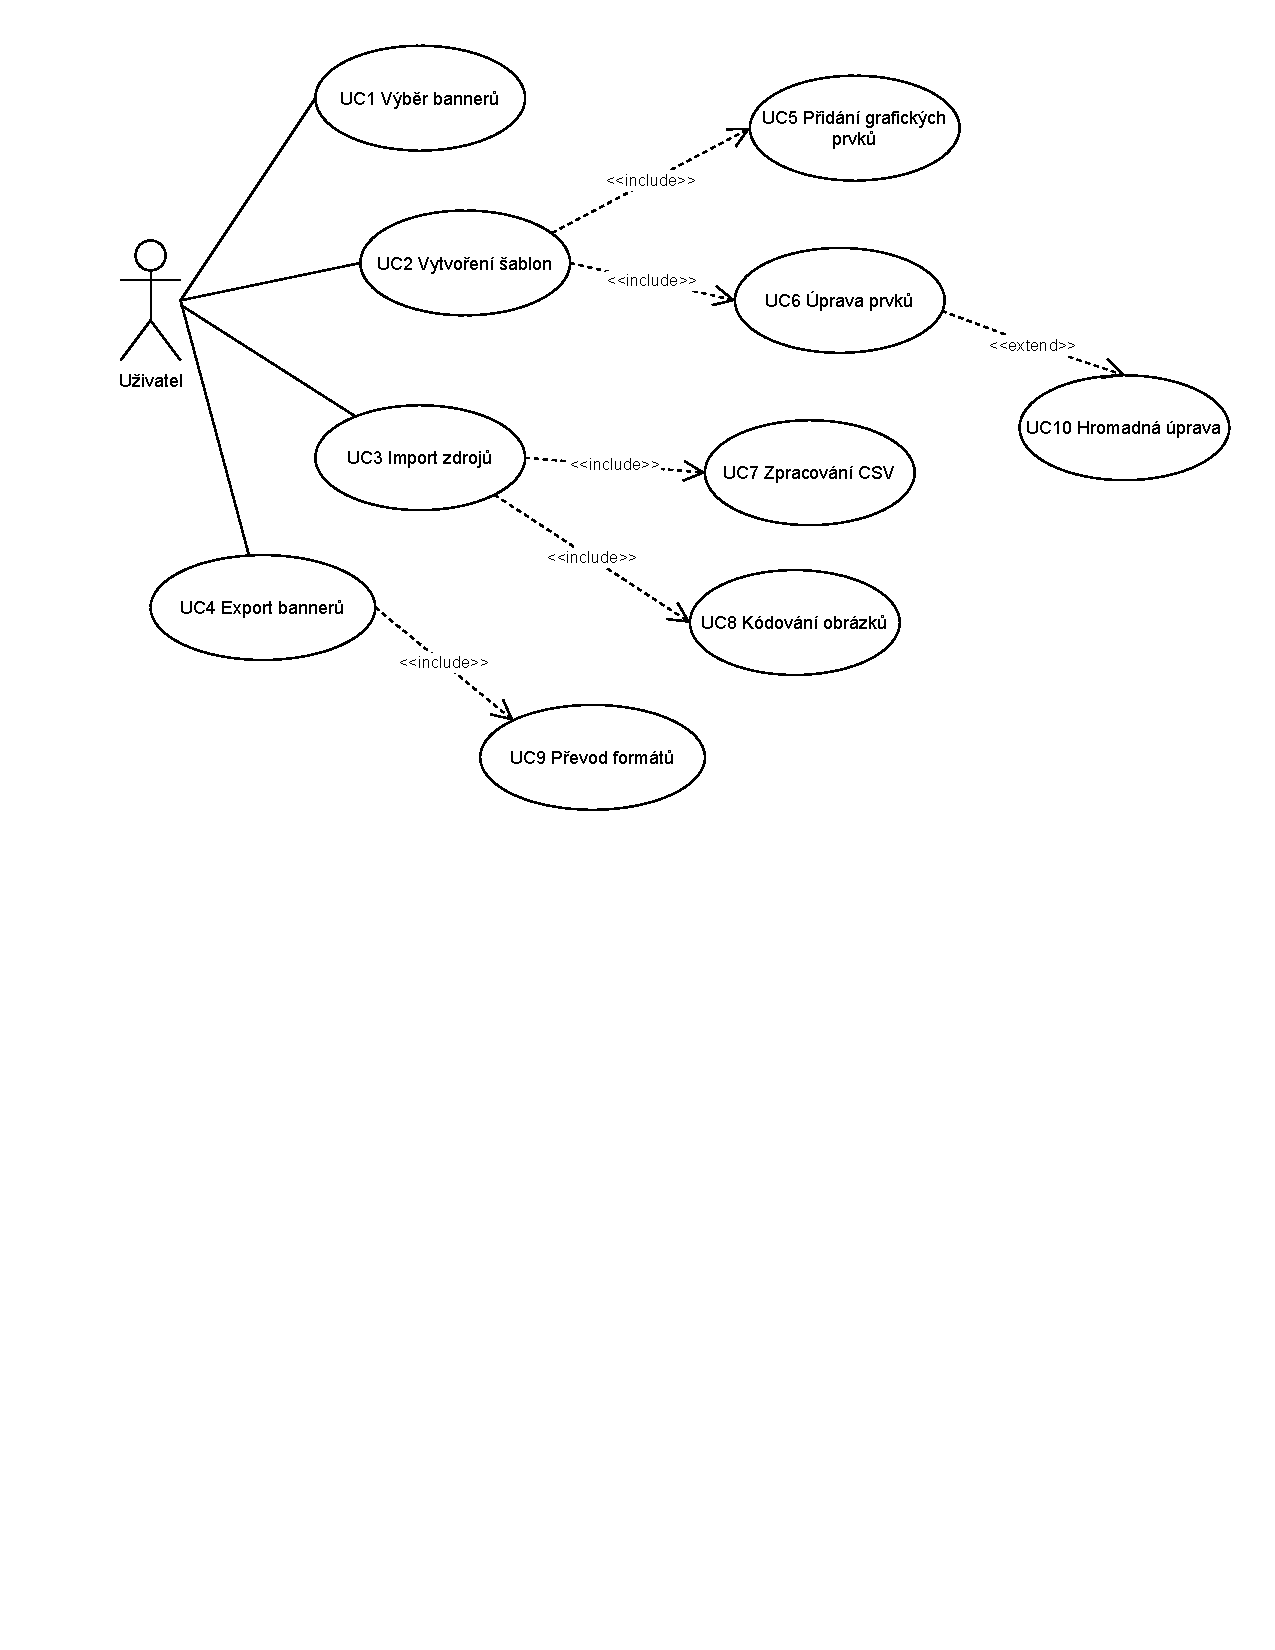
\includepdf{use-case-diagram.pdf}
    %\includesvg{}
    \begin{figure}
        \centering
        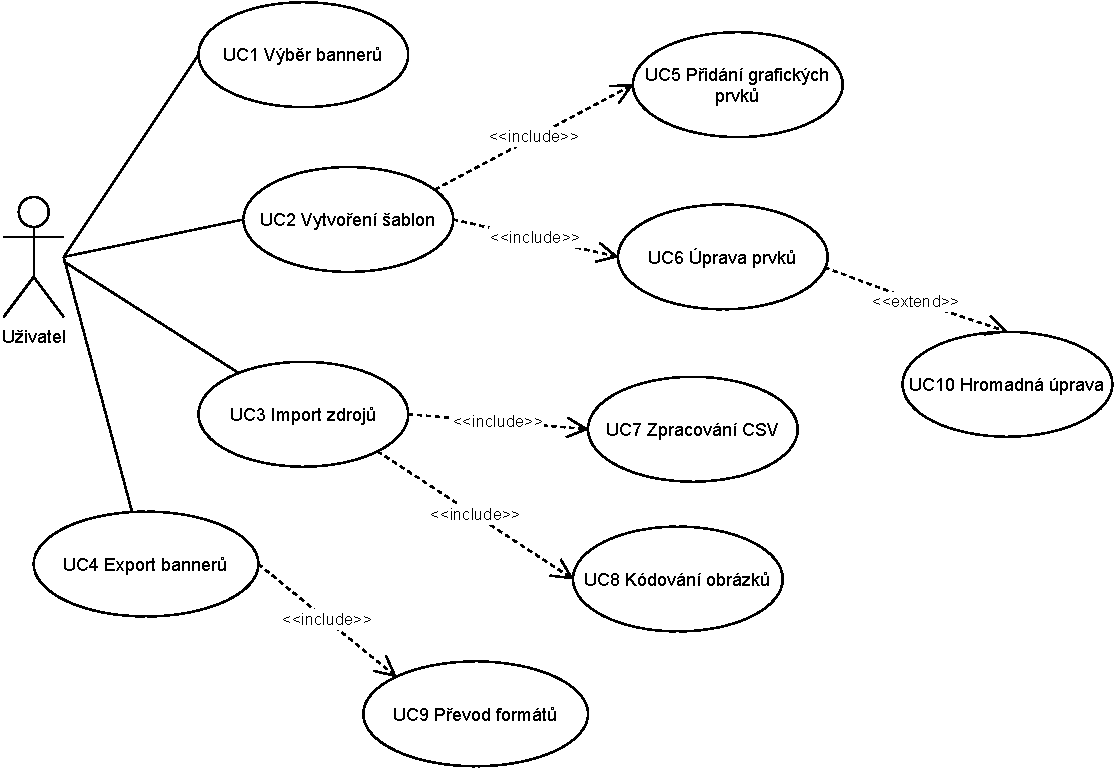
\includegraphics[width=0.85\textwidth]{Figures/use-case.pdf}
        \caption[Use case diagram]{Diagram případu užití návrhu online nástroje}
        \label{fig:use-case-diagram}
    \end{figure}

    \section{Volba technologíí}
    Moderní vývoj frontendu se ujal směrem javascriptových frameworků a knihoven. Nejvíce používanými frameworky/knihovnami se stal VueJS, Angular a React.
    Porovnávat tyto technologie by však bylo zbytečné zde rozepisovat, jelikož to není tématem této práce.
    Pro případný zájem autor doporučuje tento článek, kde jsou většina porovnání včetně benchmarků.
    Nutno podotknout, že zatímco React a Vue jsou zaměřené více na hlavní funkcionalitu a ostatní věci jako routování a state management nechávají
    na dodatečných balících. Angular většinu funkcí obsahuje v základu.
    I z tohoto důvodu a lepší znalosti frameworku Angular se autor této práce rozhodl právě pro tuto možnost. 

    Pro práci grafikou na straně prohlížeče jsou k dispozici 2 HTML elementy a tím jsou Canvas a SVG.
    Canvas, v překladu kreslící plátno, kreslí použitím rastrové grafiky. Oproti tomu SVG je kreslí vektorovu grafiku.
    Jelikož je cílem práce tvorba bannerů, do kterých má být možno vkládat fotografie, padá volba na Canvas.
    Samotný canvas ale neposkytuje moc rozšířenou funkcionalitu. Naštěstí na tento problém existuje řešení v podobě knihoven.

        \subsection{JS knihovny pro práci s Canvas elementem}
        Javascriptový ekosystém je velice rozsáhlý a je z čeho vybírat. Dostupných knihoven pro práci s canvasem je mnoho.
        Ne každá knihovna ale poskytuje potřebnou funkcionalitu,
        jelikož se zaměřuje na jiný problém. Tato část porovná pár autorem vybraných knihoven.

            \subsubsection{Fabric.js}
            První porovnávanou knihovnou je Fabric.js. Dokáže pracovat s jakýmkoli tvarem nebo vloženým obrázkem. Umožňuje na obrázky používat filtry,
            má zabudovanou podporu tvorby animací, seskupování objektů a stínování. Poradí si i při práci s textem, se kterým dokáže vykreslovat různé fonty,
            zarovnávat jej a samozřejmě měnit velikost.
            Výhodou této knihovny oproti ostatním je, že má zabudovaný parser pro konverzi do formátu SVG nebo JSON a zpět z těchto na canvas.  
            
            \subsubsection{Konva.js}
            KonvaJS je knihovna pro práci ve 2D jak pro desktopové zařízení, tak pro mobilní. Nabízí práci s textem (včetně podpory různých fontů),
            animace, geometrickými objekty, obrázky (rastrové i vektorové) a videa, filtry atd. Výsledek práce se dá exportovat jako serializovaný
            JSON nebo obrázek ve formátu PNG nebo JPEG, u kterých umožňuje zvýšit poměr pixelů pro lepší kvalitu.
            Při exportu do formátu JPEG dovoluje zvolit výslednou kvalitu. Mezi výhody spadá podpora zařízení s vysokou hustotou pixelů, a gest na mobilních zařízeních.
            Pro programátory nabízí i statické typování v podobě definicí v Typescriptu. 

            \subsubsection{Easeljs}
            Tato knihovna jako předešlé disponuje velkou škálou funkcionalit.
            Oproti ostatním ale nemá přímo zabudovanou možnost animací.
            Podporuje mobilní zařízení a do jisté míry vykreslování pomocí technologie WebGL.

            Jelikož je vysoká pravděpodobnost, že by nástroj používali grafici, je potřeba zajistit dobrou podporu pro retina displeje.
            Proto pro implementaci byl zvolena KonvaJS.

    \section{Návrh implementace}
    Základním stavebním blokem aplikací v Angularu jsou moduly. Ty logicky oddělují různé části aplikace od sebe a tím umožňuje lepší oddělení
     zodpovědností (Separation of concerns). Další 2 hlavní prvky, které pomohou k implementaci jsou komponenty a služby.  

    Komponenty spravují viditelné části uživatelského rozhraní a jejich interakci s uživatelem (vstupy, události).
    Vazba mezi viditelnými částmi HTML a komponentami je obousměrná. Díky tomu se všechny prvky rozhraní aktualizují na základě momentálního stavu aplikace,
    který je uživateli zobrazen a zároveň reaguje na jeho podněty. Navíc, komponenty lze znovu využívat a dávat jim vstupní parametry.
    Tato výhoda bude použita pro zobrazení úprav více objektů stejného typu. 

    Služby naopak slouží pro zachycení funkcionalit, které typicky nemají souvislost s uživatelským a mohou být opakovaně použity napříc aplikací.
    Přístup ke službám je zajištěn přes dependency injection (injektáž závislostí, DI). Lze je injektovat do komponent nebo ostatních služeb.
    Důležité je vědět, že injektace probíhá skrz tzv. providery. Ti říkají, v rámci čeho je služba poskytována (modul, komponent, aplikace) a
    podle toho vytvářejí instance. Jelikož vstupů, které budou ovlivňovat vykreslování bannerů na plátně bude hodně,
    byla by komunikace striktně mezi komponentami složitá. Proto bude využita sdílená služba.
    Ta má za úkol zastiňovat API vybrané knihovny a vykreslování na plátno. Díky tomu budou mít všechny potřebné komponenty přístup ke službě a
    přímo ovlivňovat vykreslené objekty.

    \begin{figure}[h]
        \centering
        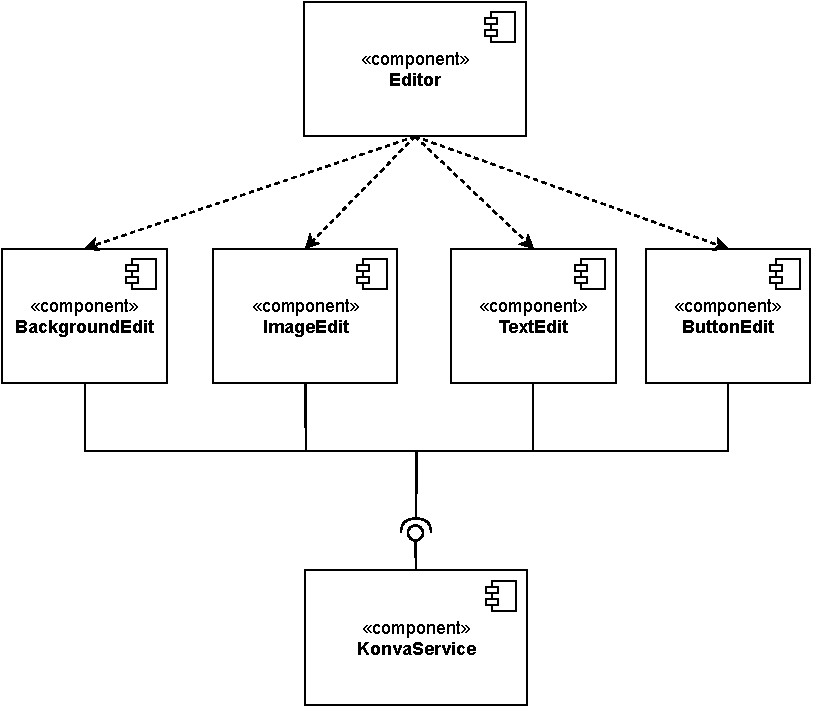
\includegraphics[width=0.85\textwidth]{Figures/component-diagram.pdf}
        \caption[Diagram komponent editoru]{Diagram komponent online nástroje}
        \label{fig:component-diagram}
    \end{figure}

        \subsection{Zobrazení více bannerů najednou}
        Aby uživatel dokázal pracovat rychle a efektivně bude mu umožněno upravovat více bannerů najednou. K docílení tohoto požadavku je možno použít
        třídu \emph{Konva.Group}. Ta umožňuje seskupení vícero objektů a jejich oříznutí.
        Každá skupina bude reprezentovat jeden banner. Oříznutím bude zajištěno zobrazení, indikující přesah okraje banneru.

        \subsection{Práce s tvary na plátně}
        Práce s tvary jako přesouvání a transformace jsou základem grafických editorů. Díky použité knihovně zajištění těchto funkcí nebude složité.
        Ale potřebou je, aby se provedená transformace projevila i na ostatních bannerech. Pro implementaci transformací lze využít třídu \emph{Konva.Transformer}.
        Ta mimo jiné poskytuje události \emph{transformstart, transform, transformend}, díky kterým bude jasné, co se s objektem děje a aplikovat stejnou transformaci i
        na stejné objekty v ostatních bannerech. Stejný postup platí i pro rotaci.

        Při přesouvání nastává událost \emph{dragmove}. K té také lze naslouchat. Naivní možnost by byla přesouvat na ostatních bannerech stejný tvar o počet pixelů,
        o které byl posouvaný tvar změněn. To ale způsobí, že na malých rozměrech by se objekt dostal rychle na hranici a na velkých rozměrech by
        změna nešla skoro poznat. Při přesouvání se musí vzít v potaz velikost přesouvaného objektu a zároveň rozměr banneru, na kterém má být přesunut.
        Jako možnost se nabízí spočítat si pozici středu objektu v procentech v závislosti na daném banneru.
        Potom si pozici pro příbuzné objekty jde snadno dopočítat.

        Pro pozicování pozadí v případě, že půjde o obrázek, bude použité jiné chování přesouvání. Místo toho, aby se vykresloval celý, bude vykreslován jen výřez.
        Pokud bude nutné zobrazit na pozadí jinou část obrázku, potáhnutím pozadí lze měnit pozici výřezu, který bude vykreslen.

        Při různých úpravách se však může stát, že některé objekty se na bannery menších rozměrů nevlezou nebo budou muset být jinak upraveny.
        Proto bude umožněno je odebrat nebo individuálně upravit.

        \subsection{Úpravy textu}
        ext je na banneru velice důležitý. Z tohoto důvodu by měla editace textu nabízet obvyklé prvky jako výběr fontu.
        Pro možnost širokého výběru bude zajištěno napojení na Google Fonts a tím i zpřístupněny všechny fonty, jenž Google poskytuje.
        Dále pro text budou možnosti jako je zarovnání textu, zalamování, kurzíva, tučný text, změna barvy a stínování pod textem.
        Vykreslování stínů na canvasu v prohlížeči je výpočetně složitá operace. K urychlení lze použít schopnost knihovny Konva.js uložení v mezipaměti,
        což převede celý text i se stínem na obrázek,
        který je jednodušší vykreslit. Při následné jakékoliv změně textu se mezipaměť přepíše novými hodnotami.

        \subsection{Nahrávání obrázků}
        Cílem je práci usnadnit co nejvíce a umožnit nahrání jak ze vzdálených zdrojů, tak i z lokální pracovní stanice.
        Obvykle by se obrázky a fotografie nahráli na server, odkud by již byly dostupné uživateli kdykoli by je potřeboval.
        Tohle jsou však další rozšířené funkce, které tato práce svým rozsahem neřeší. Proto bude nahrávání řešeno pomocí kódování base64,
        které umí binární data převést na ASCII znaky. Tento přístup je nutné použít i v případě nahrání ze vzdálených zdrojů Internetu.
        Dle specifikace HTML, načítání obrázků z jiné domény do canvasu způsobí tzv. zkažený (tainted) canvas, který není možné exportovat.
        Další způsob je povolení \emph{CORS} ze strany zdrojového serveru. Díky tomu by se obrázky mohli načíst bez nutnosti kódování.

        \subsection{Exportování výsledků}
        Stejně jako nativní HTML canvas, Konva.js poskytuje možnost exportování ve formátech JPG a PNG.
        Výsledek za zakódován v base64, který už však není problém zobrazit nebo stáhnout.
        Není potřeba však exportovat celé pracovní plátno, ale jen potřebné bannery. Ty, jak je již bylo zmíněno,
        jsou pouhým seskupením různých objektů. Pro zařízení s vyšší hustotou pixelů je dostupná možnost exportovat se zvýšeným poměrem pixelů (pixel ratio). 

        Zde ovšem je potřeba zajistit, aby výsledný export byl v co nejvyšší kvalitě a zároveň nejmenší velikosti.
        Preferovaný formát při exportu bude PNG, jelikož je bezztrátový. Pokud by výsledný soubor přesahoval 150 KB,
        další možností je použít 24bitový formát PNG-24.
        Ten neuchovává informace o průhledném alfa kanálu a tím na každý pixel ušetří 1 bajt, celkově tedy je možná úspora až 25\% původní velikosti. 

        Alternativou k těmto formátům je nový formát speciálně vytvořený pro web. Tím je formát WebP, vyvíjený společností Google.
        Dle oficiálních zdrojů podporuje ztrátovou i bezztrátovou kompresi. Přičemž v porovnání v PNG dokáže smrsknout až o 26\% lépe a v porovnání
        s JPEG dokonce až o 34\%. Podpora zobrazení tohoto formátu je rozšířená na všechny nejvíce využívané webové prohlížeče.
        Kromě Facebooku, stále mnoho reklamních systémů, včetně Googlu samotného, tento formát nepodporuje.

        \subsection{Ukládání projektu}
        Projekt se všemi úpravami půjde uložit do souboru. Ten bude obsahovat potřebná data ke znovuvytvoření identické stavu, jako byl před uložením.
        Díky této funkci uživatelé nepřijdou o veškerý postup, který udělali.

    \section{Datové struktury}
    Při nahrávání datasetů je potřeba nějakým způsobem uložit nahraná vstupní data. Jelikož online editor musí být schopný upravovat šablonu i dataset,
    musí se pro každý objekt na plátně ukládat i jeho stav. V každém datasetu budou uchovávány informace o bannerech, které se mají vykreslit.
    A pro každý banner musí být uložen momentální stav jednotlivých objektů. Tohoto lze docílit serializací vykreslených uzlů.
    Konva.js se serializací tvarů počítá, a proto ukládá pouze změněné vlastnosti. V případě budoucího rozšíření, by bylo vhodné taková data ukládat spíše do
    dokumentových NoSQL databází jako je například MongoDB a využít tak možnosti vnořených kolekcí dokumentů. 

    Uchováváním těchto dat v paměti bude zajištěno, že každý banner v jakémkoli datasetu bude moct být opětovně správně vykreslen.

    \section{Návrh uživatelského rozhraní}
    Rozhraní grafických editorů musí být intuitivní. Podobné nástroje už existují dlouhou dobu a jejich uživatelé mohou být zvyklí na pojmenování určitých funkcí
    nebo znázornění ikonkou. Proto je třeba, aby i implementovaný nástroj se vzhledem blížil nebo podobal zavedenému de facto standardu grafických editorů. 

    Součástí prostředí bude horní lišta. Ta bude mít na levé straně tlačítko pro hlavní nabídku. Součástí nabídky budou položky pro:
    \begin{itemize}
        \item export všech bannerů,
        \item uložení do souboru.
    \end{itemize}
    Na pravé straně lišty půjdou najít možnosti lokalizace. Implementace nástroje v rámci této práce bude lokalizována do 2 jazyků. Těmi jsou čeština a angličtina. 

    Editor bude mít 2 postranní sloupce mezi kterými se bude nacházet pracovní plátno. Levý sloupec bude obsahovat seznam šablon,
    které se budou moct přehazovat a přejmenovávat. Vedle seznamu také budou dostupné některé základní nástroje pro kreslení tvarů.
    Na pravém sloupci budou zobrazeny všechny tvary a objekty, které se momentálně nachází na bannerech, po položkách.
    Jednotlivé položky půjdou rozkliknout a zobrazí se vlastnosti objektu, jenž půjdou změnit.

    \begin{figure}[ht]
        \centering
        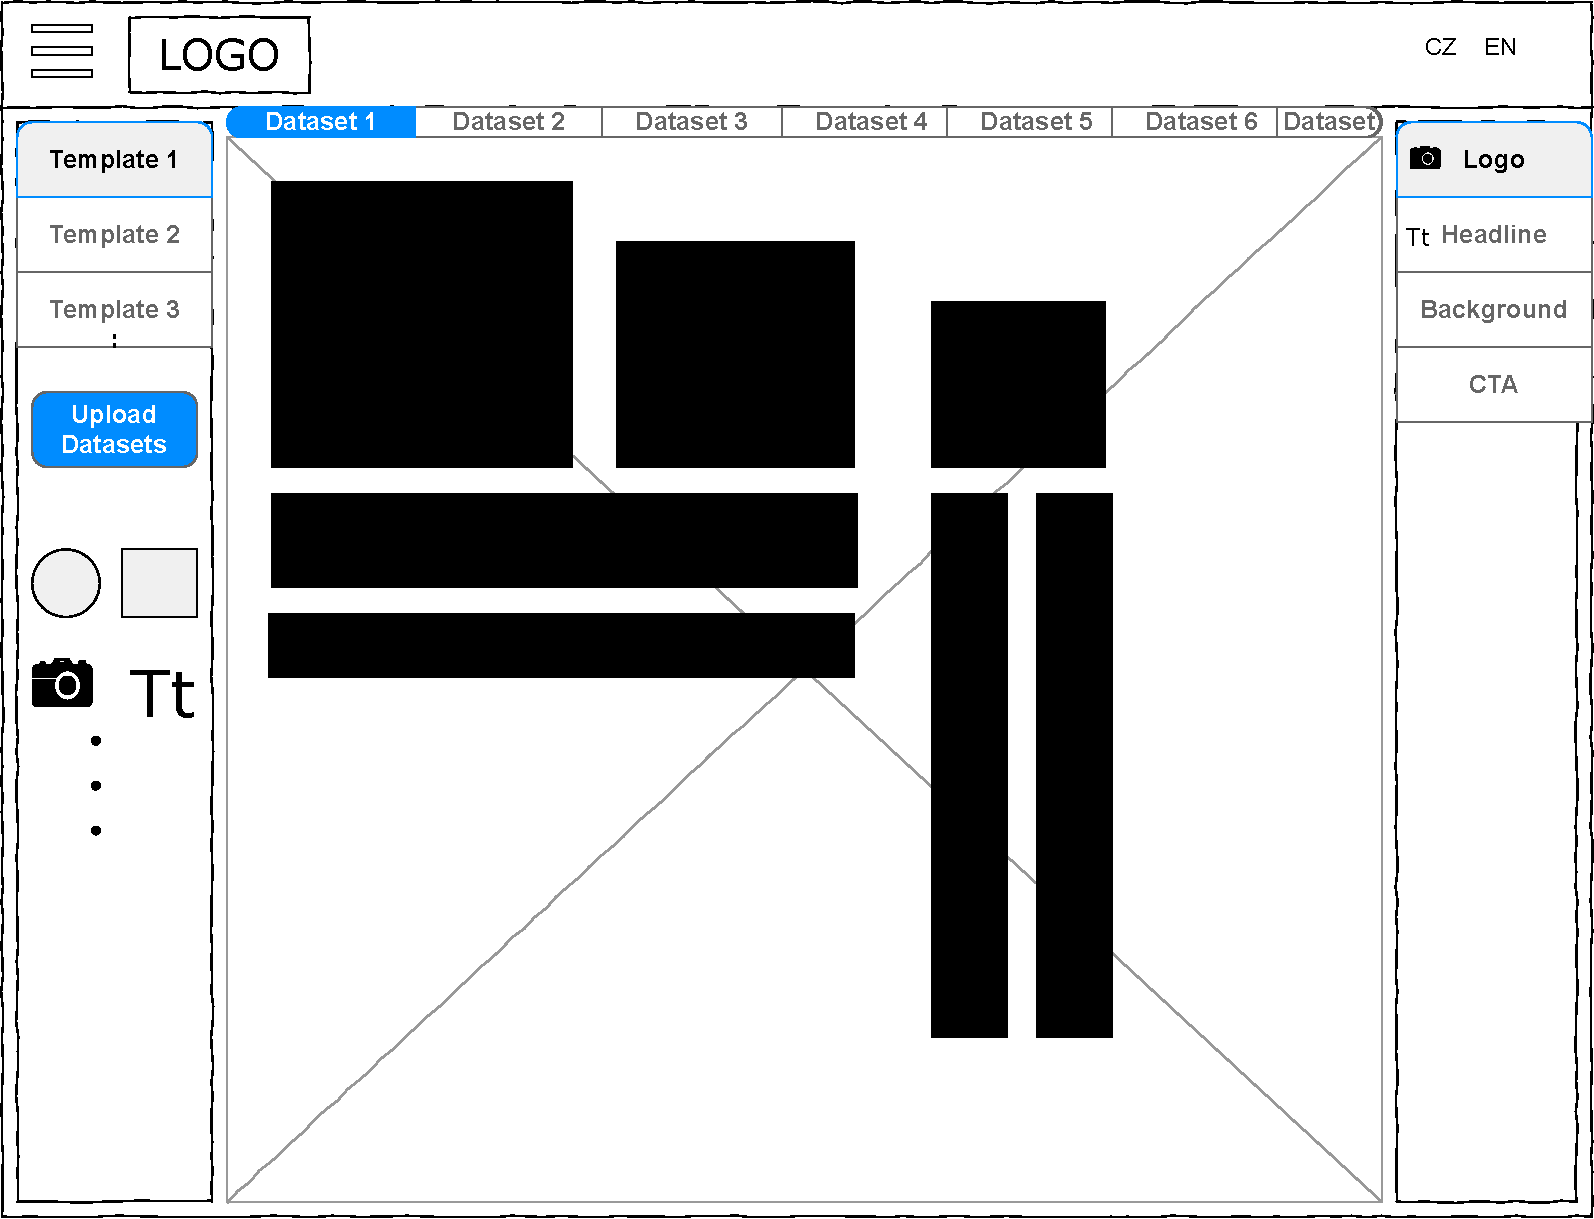
\includegraphics[width=0.8\textwidth]{Figures/wireframe.pdf}
        \caption[Wireframe UI]{Návrh uživatelského rozhraní ve formě wireframu}
        \label{fig:ui-wireframe}
    \end{figure}

        \subsection{Text}
        Výběr fontů bude implementován způsobem vyhledávání s automatickým zobrazením nebližších shod.
        Textové sdělení jako takové půjde vložit přes textovou oblast. Barva bude vybírána skrze samostatnou komponentu, kde barva půjde zadat buďto
        ve složkách RGB nebo jako HEX řetězec nebo bude moct být vybrána. K barvě je i možný alfa kanál.
        Zarovnání textu, ztučnění, kurzíva, podtržení a přeškrtnutí budou jednoduchá tlačítka, která budou indikovat, zda jsou aktivní nebo ne,
        a to změnou pozadí. Výška řádku a mezera mezí písmeny budou měnitelné přes posouvátko.

        \subsection{Obrázkové filtry}
        Jelikož u některých filtrů jde změnit \enquote{síla} účinnosti (např. kontrast, zesvětlení, posterizace, \ldots), bude možné ji měnit jako posouvátko.
        Ostatní filtry, které mají stav pouze vypnuto/zapnuto (invertování barev, stupně šedi), bude možno aktivovat pomocí přepínače.

        \subsection{CTA}
        Tlačítko pro vyzvání k akci je kombinací textu a jednoduchého tvaru na pozadí. Stylizace bude rozdělena na 2 záložky, kde jedna je pro úpravu textu a
        druhá pro úpravu pozadí. Pro CTA bude možnost zaoblení rohů.

        \subsection{Export}
        Exportování výsledků bude provedeno v rámci dialogového okna v krocích, které postupně navedou uživatele.
        Prvním krokem bude výběr výsledného formátu. V případě, že bude jednat o JPEG, zobrazí se i volba nejvyšší možné kvality.
        Druhý krok bude výběr datasetů k exportu, ze kterých půjdou vybrat třeba jen určité bannery. Třetím a zároveň posledním krokem je
        samotné stažení bannerů v archivu. 




\endinput
\chapter{Implementace webové aplikace}
\label{chap:implementation}

Vytvořený nástroj je editor ve formě webové aplikace. Ke zformování byly použité výše popsané technologie Angular a Konva.js. 
Jedná se o tzv. \emph{single page application (SPA)}, kde veškerý obsah a funkcionalita se nachází pouze na straně klienta a neexistuje žádný
serverový backend. Řízení stavů je vyřešeno pomocí sdílené služby, která uchovává potřebná data k vykreslování objektů na plátno.
Stavy jsou při každém potřebném překreslení aktualizovány. Díky tomuto lze celý projekt jednoduše uložit do souboru a kdykoli znovu načíst.
    
\section{Vykreslování plátna}
    O vykreslování se stará několik služeb frameworku Angular dohromady. Důvod je ten, že k určitým objektům je nutno změnit způsob jakým jsou vytvořeny a vykresleny.
    Informace o tom, co se má vykreslit, jsou jim předávány přes komponenty, které mají služby v sobě injektované. Tyto komponenty reagují
    na změny v rozhraní provedené uživatelem a jsou ihned reflektovány na plátno.

\section{Práce s aplikací}
    Uživatelské rozhraní se podobá návrhu a je vytvořeno tak, aby bylo pro uživatelé co nejpřívětivější a líbivé.
    Ukázku práce s aplikací se nachází v příloze této práce.
    Při spuštění aplikace se uživateli zobrazí dialogové okno s výběrem velikostí bannerů (obrázek \ref{fig:editor:banner-dialog}). Po vybrání se náhledy bannerů vykreslí na plátno.
    První co uživatel upravuje je šablona, do které lze ihned umístit 4 základní prvky -- pozadí, logo, titulek a CTA (obrázek \ref{fig:editor:editor}).
    Při práci s prvky (jako je např. škálování a přetahování) na jednom banneru
    se tyto akce na daném prvku provádějí i na všech ostatní bannerech (obrázky \ref{fig:editor:before-move} a \ref{fig:editor:after-move}).
    Toto chování usnadňuje a urychluje celkovou tvorbu.
    Pro drobné úpravy si může uživatel tuto funkci vypnout.
    Dále je možno přidat na bannery více textů, obrázků, kruhů nebo čtverců. Dvojitým klikem na čtverec se z něj stane mnohoúhelník, který lze libovolně upravovat
    přidáváním nebo odebíráním bodů (obrázek \ref{fig:editor:polygon}). Pokud je potřeba některé objekty zobrazovat pouze na určitých bannerech, je toto nastavení taktéž umožněno (obrázek \ref{fig:editor:options}).
    Nástroj pro všechny objekty poskytuje možnosti úprav popsané v sekci \ref{sec:implementation-design}.

    \begin{figure}[h]
        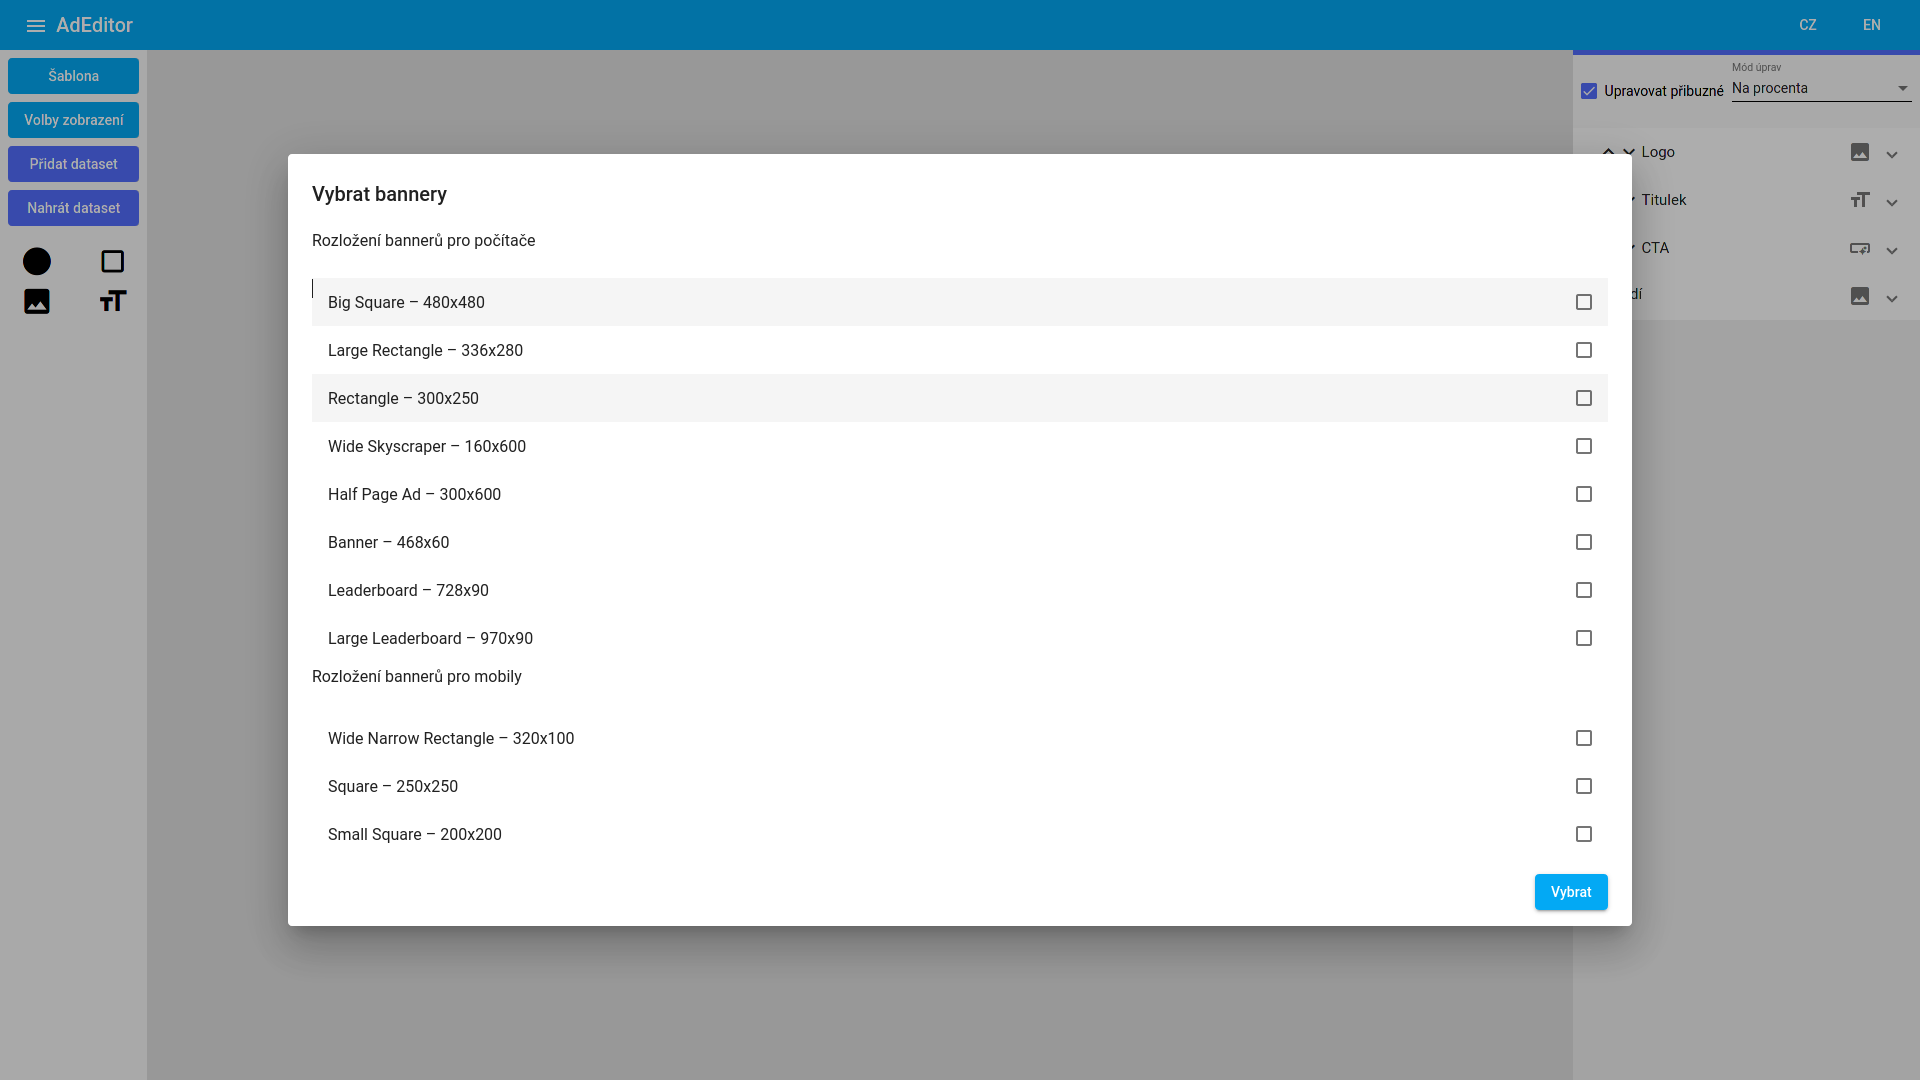
\includegraphics[width=1.0\textwidth]{Figures/editor/bannery-dialog.png}
        \caption[Výběr bannerů]{Dialogové okno pro výběr bannerů}
        \label{fig:editor:banner-dialog}
    \end{figure}

    \begin{figure}[h]
        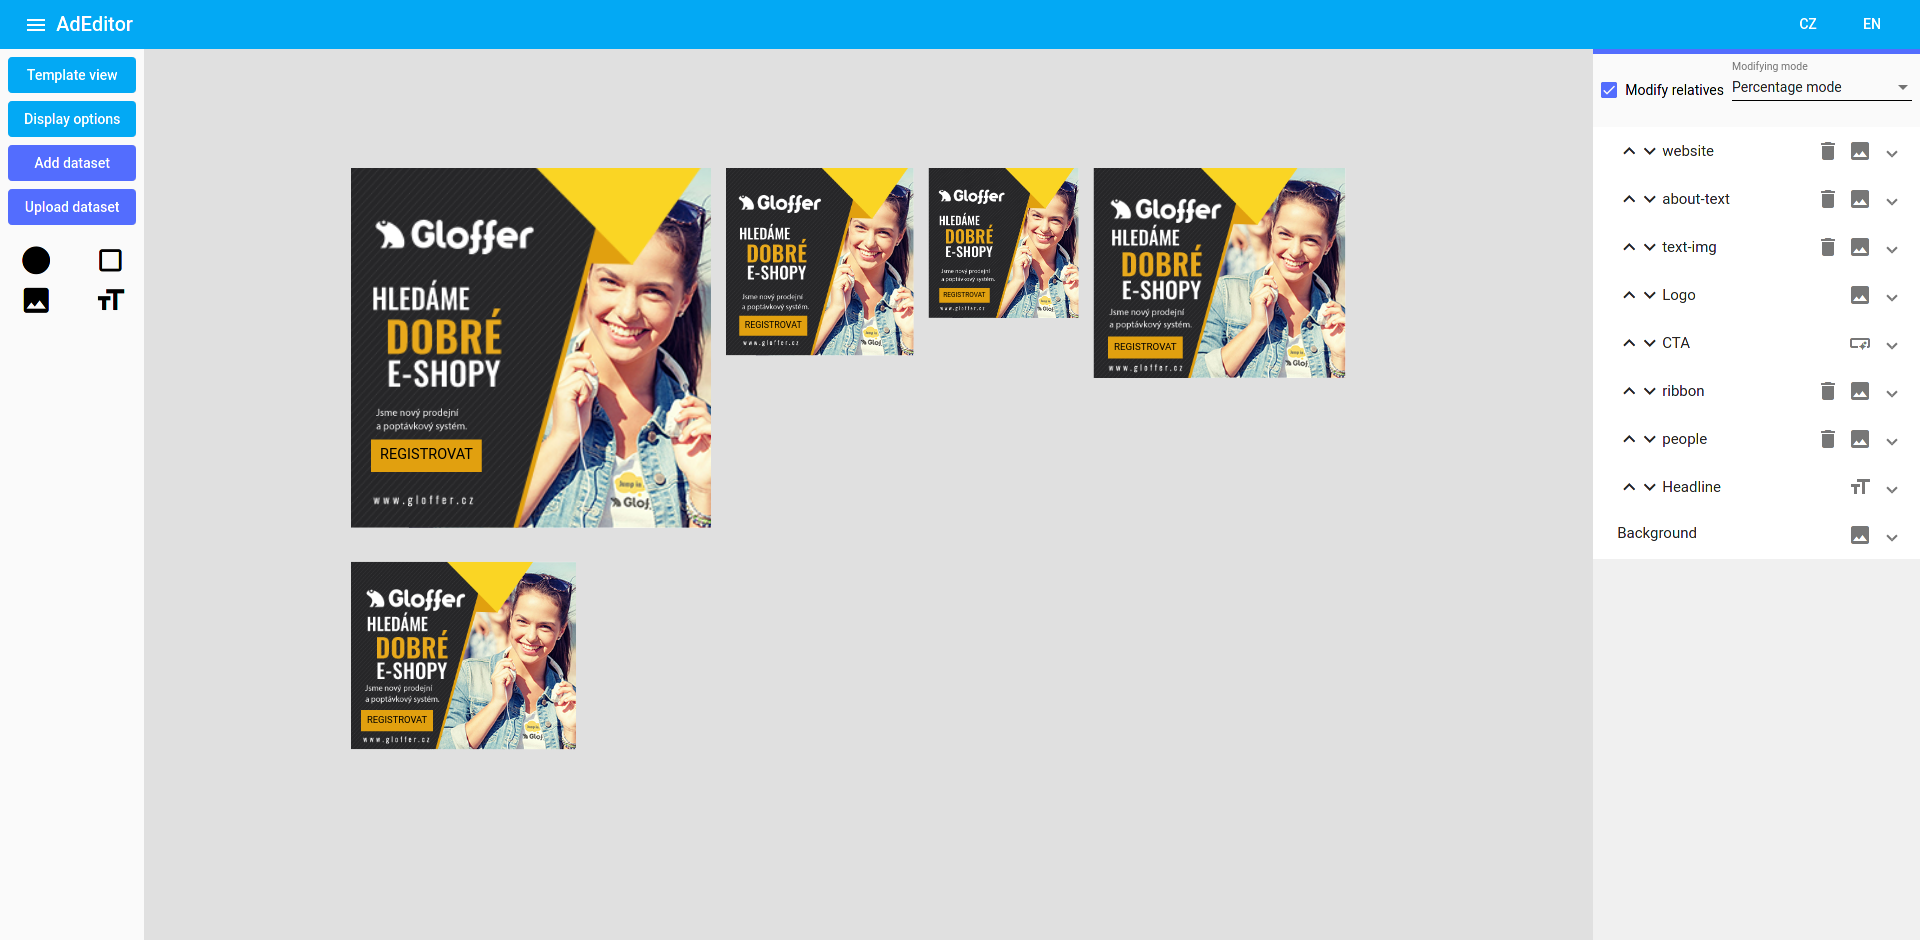
\includegraphics[width=1.0\textwidth]{Figures/editor/ad-editor-ui.png}
        \caption{Prostředí editoru}
        \label{fig:editor:editor}
    \end{figure}

    \begin{figure}[ht]
        \centering
        \begin{minipage}{.45\linewidth}
            \centering
            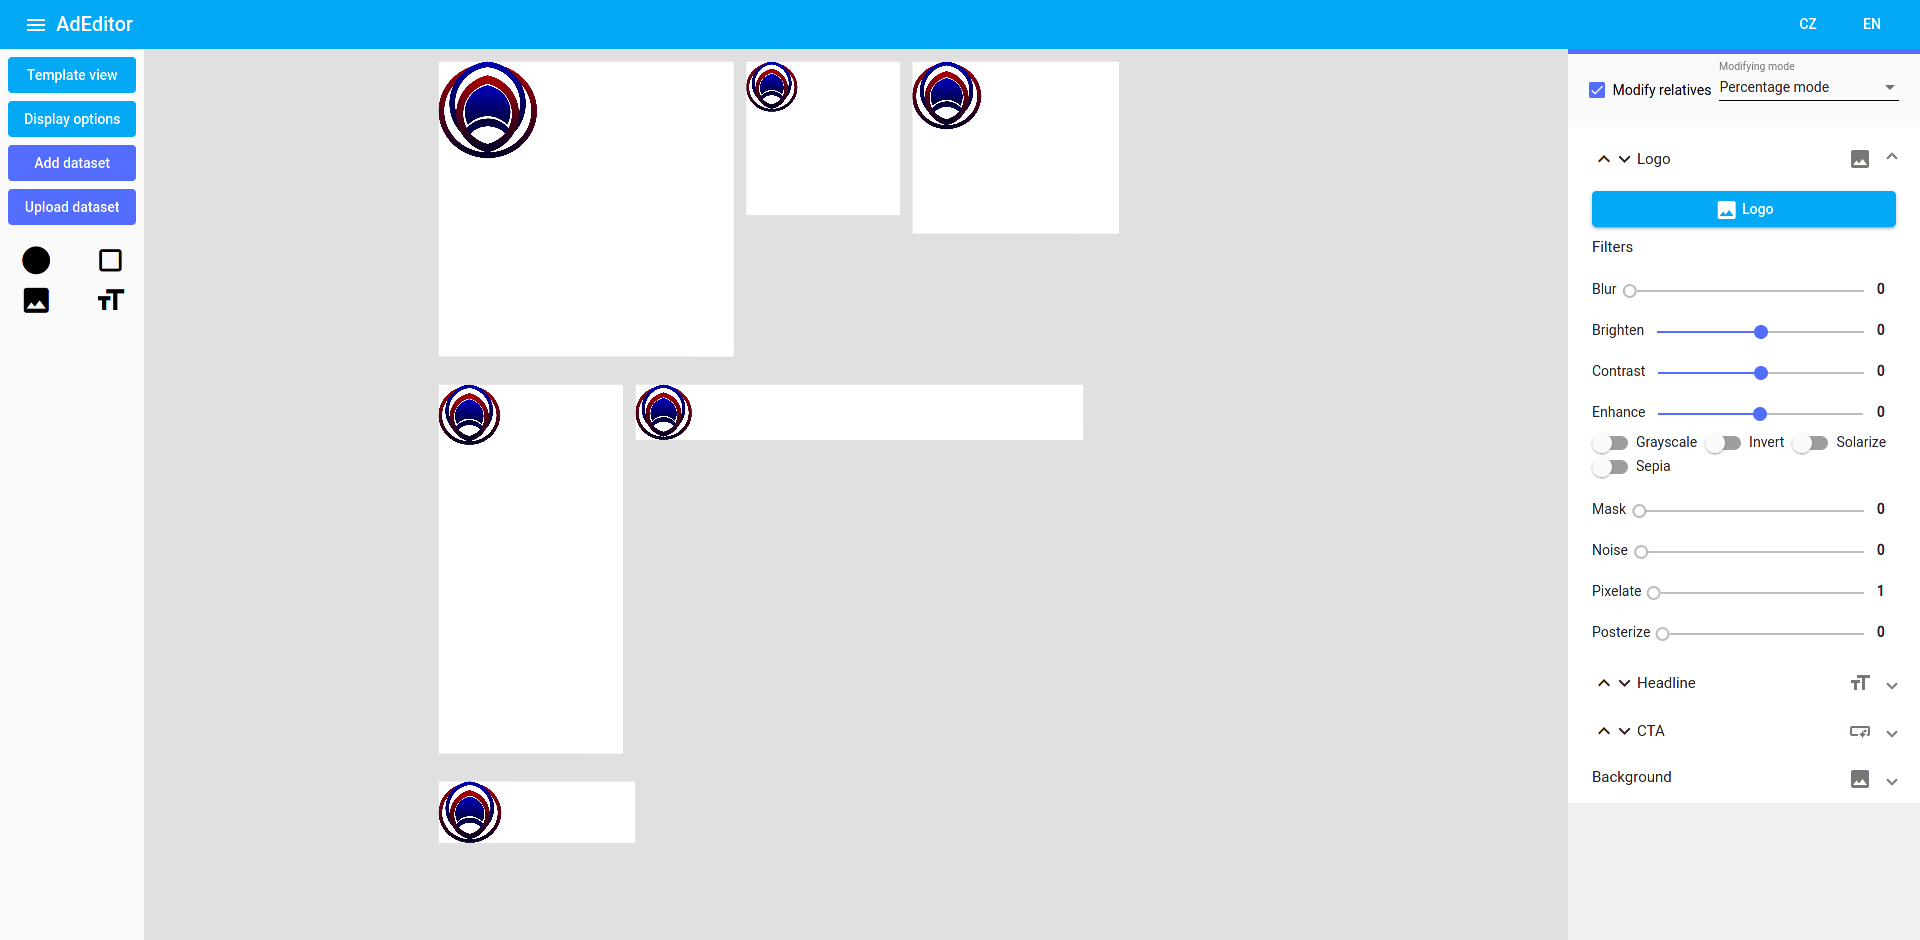
\includegraphics[width=1\textwidth]{Figures/editor/before-move.png}
            \caption{Stav před přetažením}
            \label{fig:editor:before-move}
        \end{minipage}
        \begin{minipage}{.45\linewidth}
            \centering
            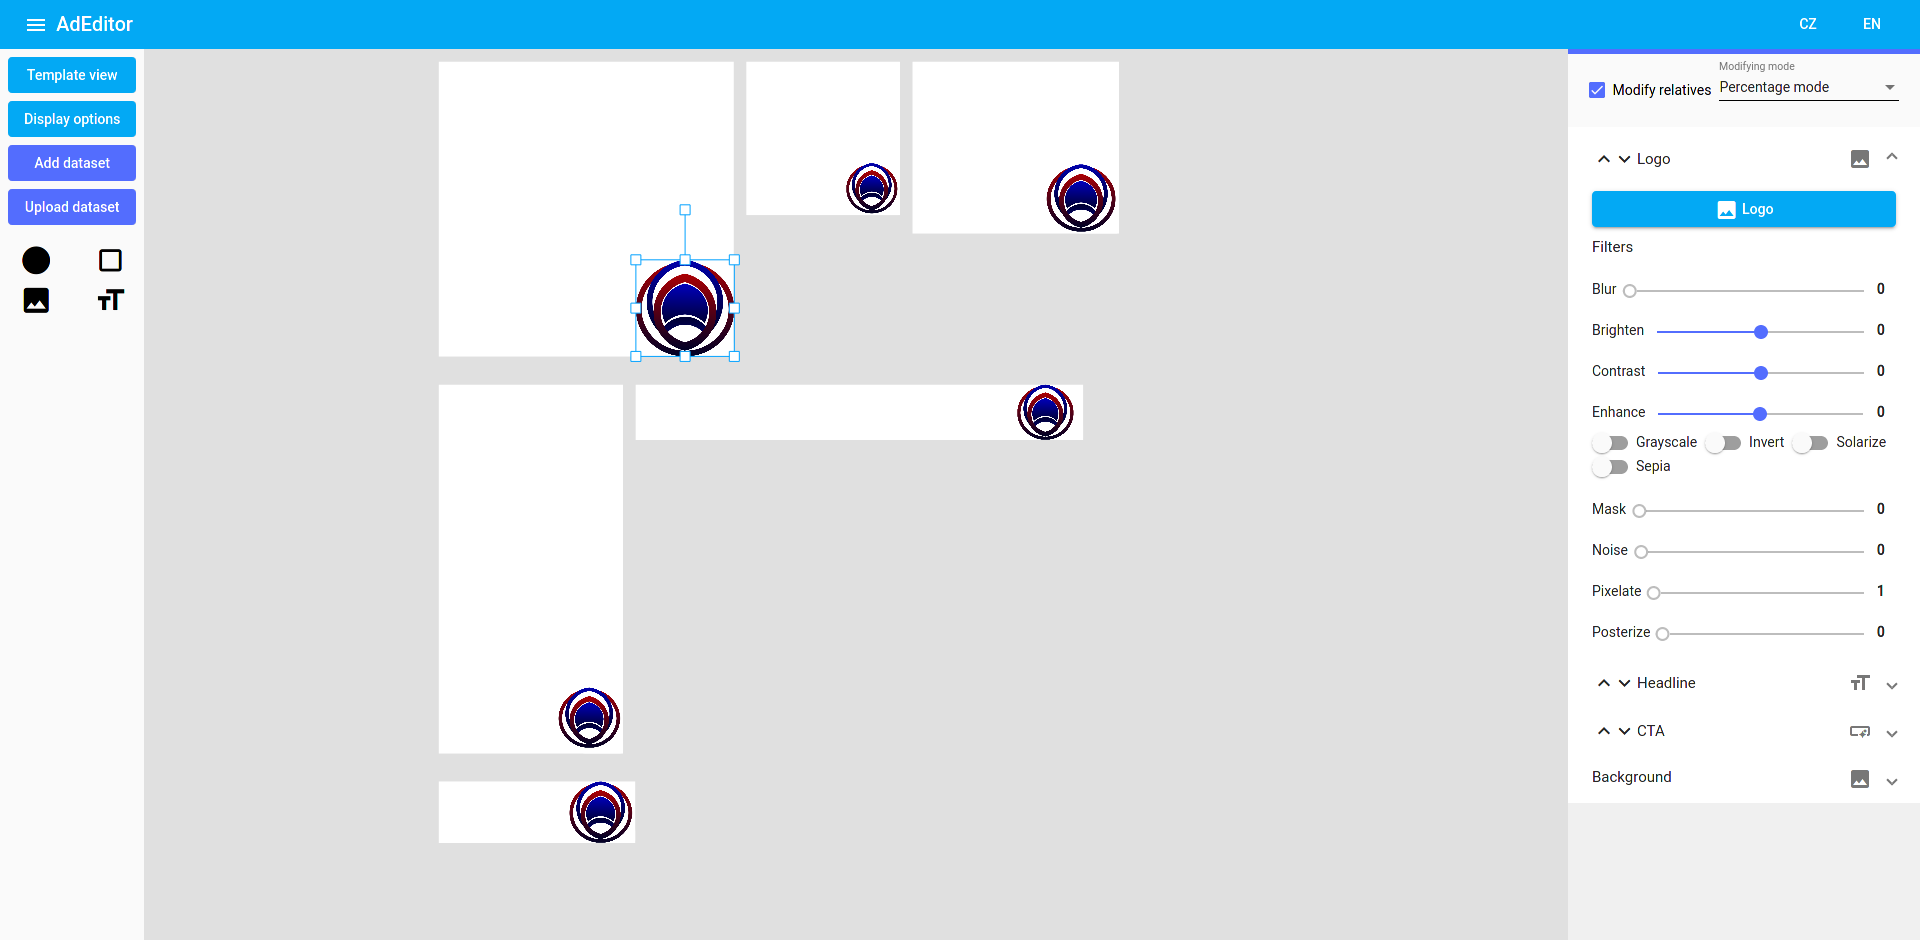
\includegraphics[width=1\textwidth]{Figures/editor/after-move.png}
            \caption{Stav po přetažení}
            \label{fig:editor:after-move}
        \end{minipage}
    \end{figure}

    \begin{figure}[h]
        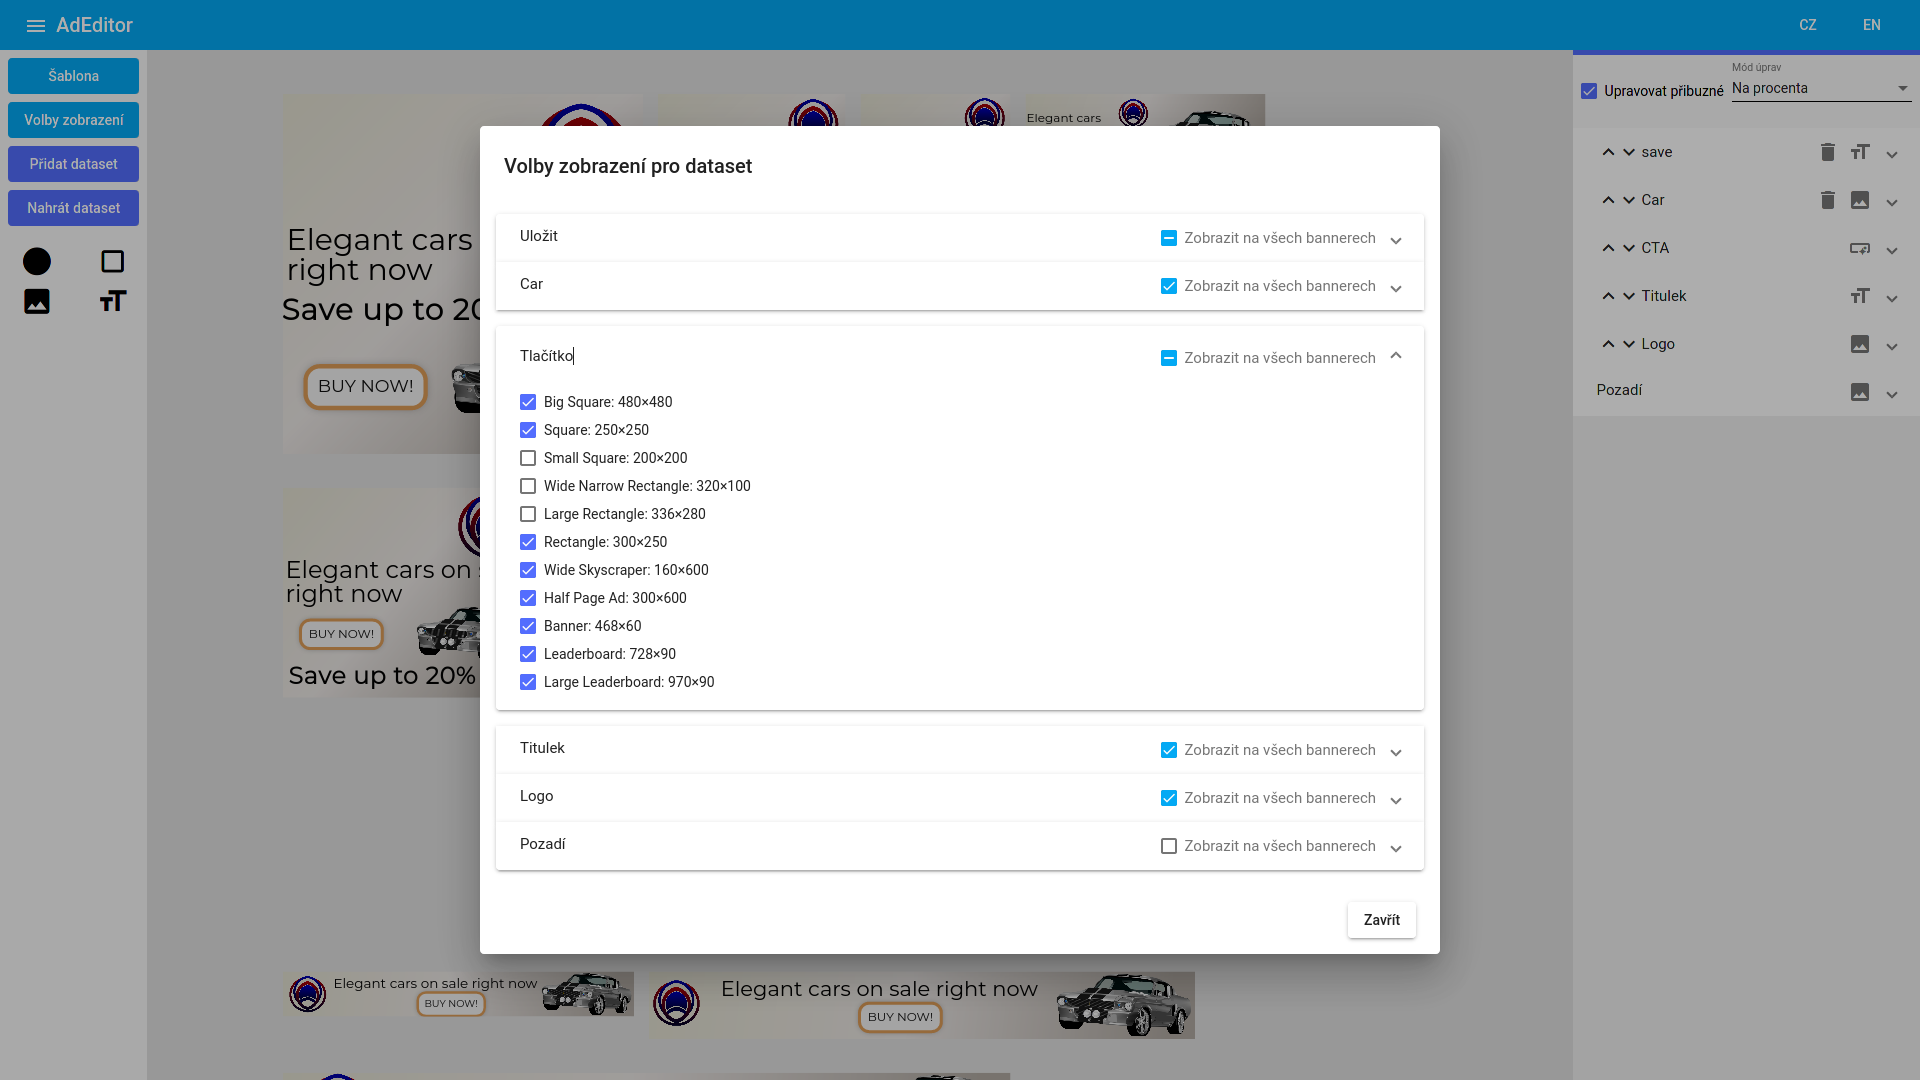
\includegraphics[width=1.0\textwidth]{Figures/editor/volby-zobrazeni.png}
        \caption[Volby zobrazení prvků]{Volby zobrazení na různých bannerech}
        \label{fig:editor:options}
    \end{figure}


    \begin{figure}[h]
        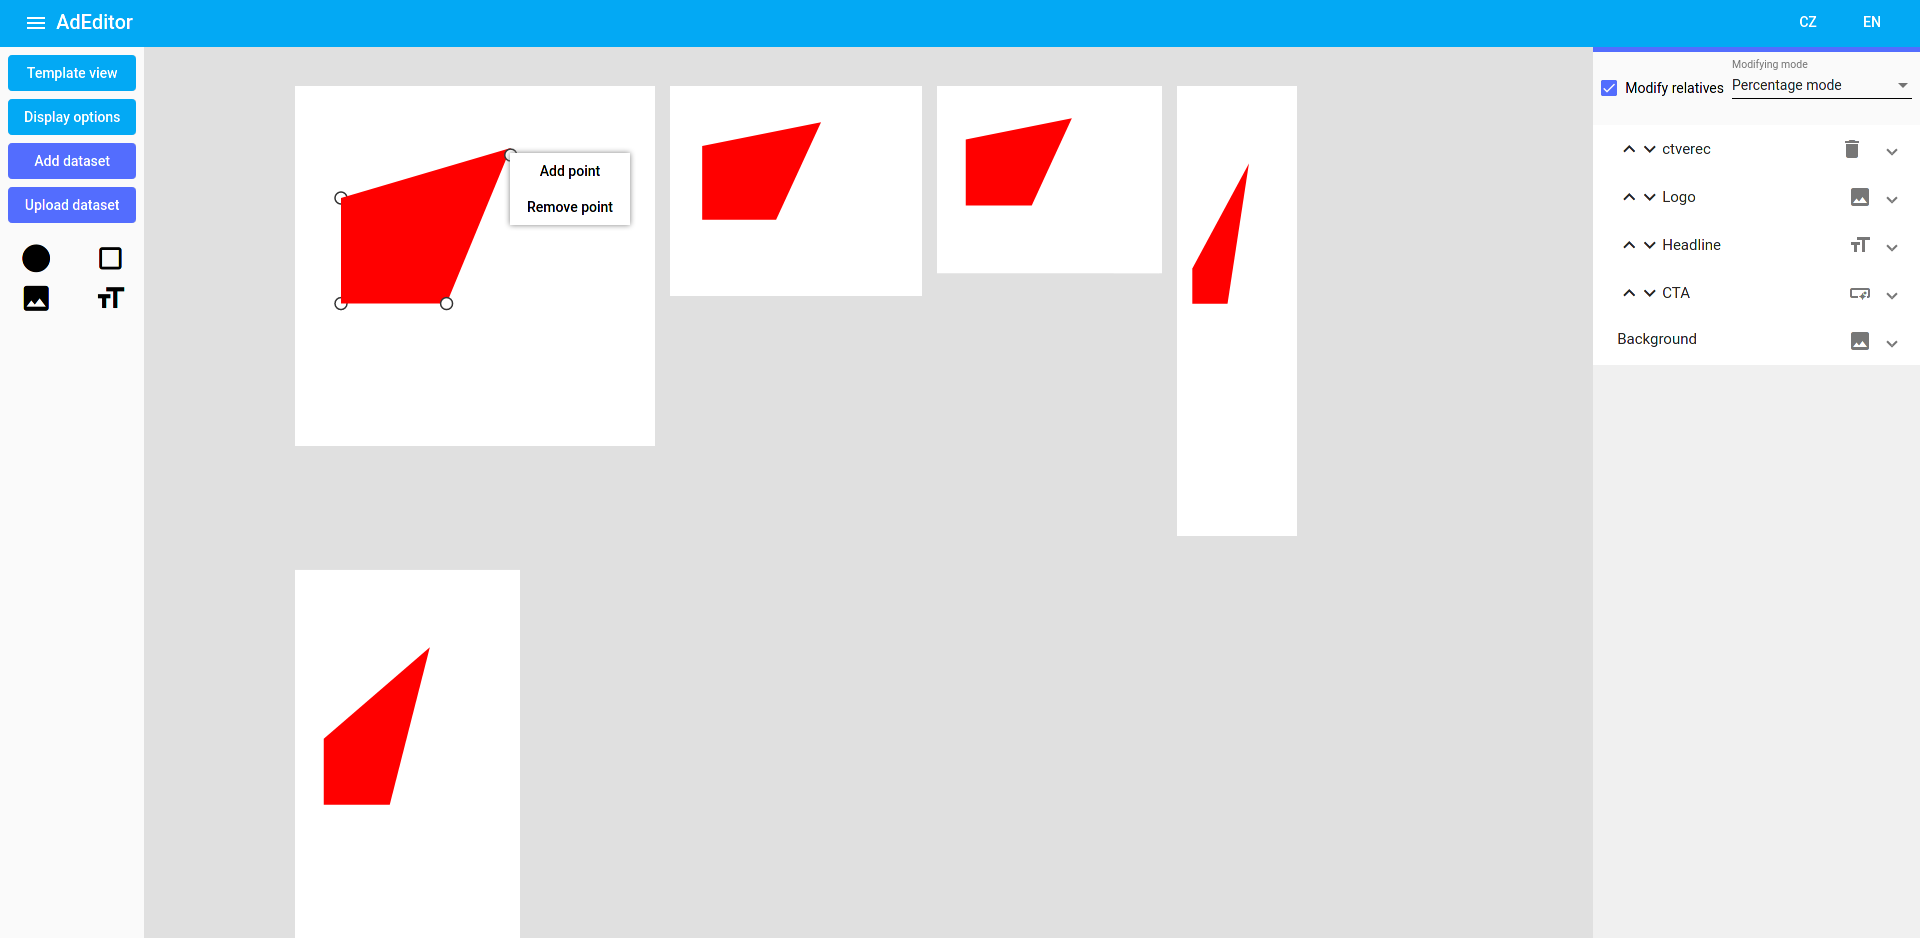
\includegraphics[width=1.0\textwidth]{Figures/editor/polygon.png}
        \caption{Úpravy mnohoúhelníku}
        \label{fig:editor:polygon}
    \end{figure}

\section{Nahrávání datasetů}
    Všechny vykreslované objekty musí být unikátně pojmenované.
    Poté je možno nahrát dataset ve formátu CSV. Jako hlavička CSV souboru musí být uvedeny názvy objektů, které si uživatel přeje změnit, v tzv.
    \emph{slugu}\footnote[2]{Slug je označení unikátního řetězce psaného malými písmeny a mezery nahrazené pomlčkou}. Měněné objekty mohou být pouze texty nebo zdroje obrázků. Obrázky aplikace umožňuje načítat i ze vzdálených zdrojů skrz 
    URL adresu, ale vzdálený server musí povolit \emph{CORS}. Po úspěšném nahrání se do aplikace tyto datasety přidají a lze mezi nimi přepínat. Každý
    dataset smí být individuálně dále upravován.

\section{Export bannerů}
    Jakmile je uživatel s výsledkem spokojen, umí bannery exportovat. Po zvolení exportu se zobrazí dialogové okno (obrázek \ref{fig:editor:exporting}) s nastavením exportu.
    Uživatel si může vybrat datasety k exportování, zda chce exportovat i šablonu, výstupní formát a případně poměr pixelů.
    Podporované výstupní formáty jsou JPEG a PNG. Pokud je zvolen JPEG, lze změnit i výslednou kvalitu.
    Dialog také zobrazuje největší odhadovanou velikost souboru, aby si uživatel nastavil vyhovující formát, případně kvalitu.
    Následně jsou vybrané datasety exportovány a staženy v ZIP archivu.

    \begin{figure}[h]
        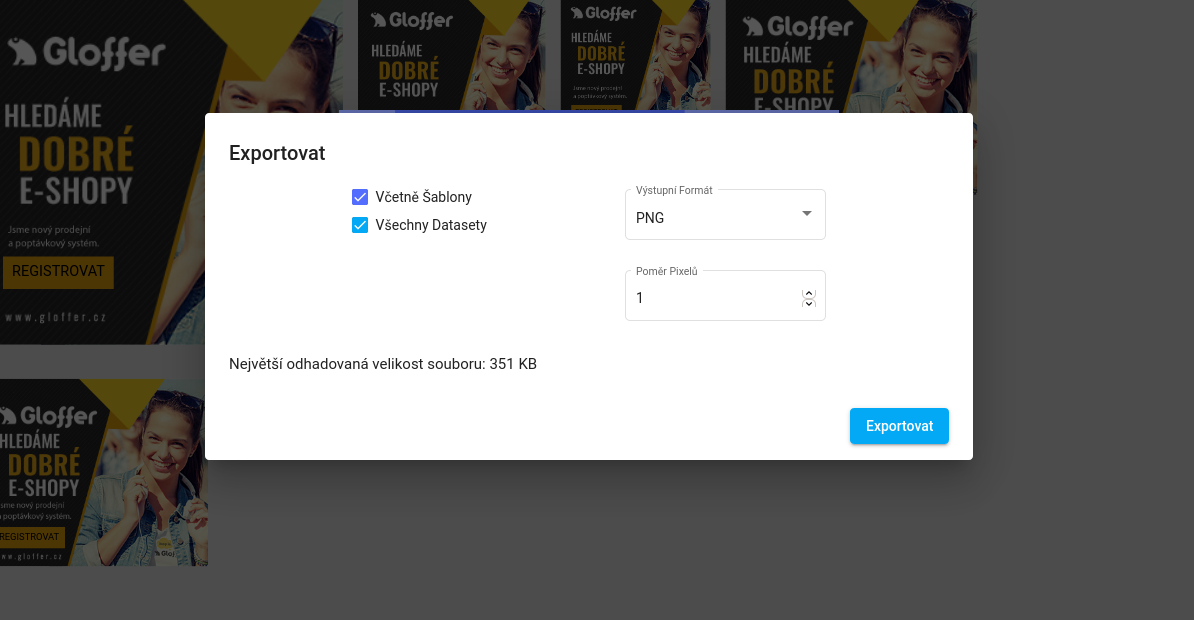
\includegraphics[width=1.0\textwidth]{Figures/editor/export.png}
        \caption{Dialogové okno pro export výsledných bannerů}
        \label{fig:editor:exporting}
    \end{figure}




\endinput
\chapter{Možná vylepšení}
\label{chap:future}
Z podstaty řešeného problému toutu prací lze najít spoustu dalších možných vylepšení. V dnešní době, kdy je drtivá většina webových
aplikací je nabízená modelem \emph{Software as a Service (SaaS)} by se i řešení této práce dalo nadále upravovat podobným směrem.
V této kapitole autor práce popisuje několik možností, jak by se výsledný software dal dále zdokonalit.

\section{Editor}
Samotný editor již nabízí uživateli řadu potřebných funkcí. Budoucí iterace by mohli práci ještě usnadit a zlepšit. Jeda z prvních schopností
editoru, kterými by mohl v budoucnu disponovat je seskupování objektů. Další užitečná funkce je přichytávání taženého prvku na základě 
ostatních tvarů, které se na banneru nacházejí. Při práci se složitějšími designy, by se právě tyto funkce uživateli hodili.
Následně už složitějším vylepšením by bylo přidání časové osy a animací. Samotná použivá knihovna pro práci s canvasem, Konva.js, umožňuje základní
prvky animací jako je pohyb, škálování, rotace, změna barev apod. Přidání tohoto by také znamenalo možnost exportu do jiného formátu umožňující 
než pouze JPEG a PNG. Nabízí se možnost exportu do formátu GIF nebo HTML banneru.

\section{Backend}
Momentální aplikace je celá řešená pouze na straně prohlížeče uživatele a neposkytuje žadný backend. Přidáním této části k aplikaci se otevírají
další možnosti využití. Ukládání uživatelských projektů na server, ukládání šablon, nahrávání fotek a obrázků, případně i vytváření celých reklamních 
kampaní. Autentizace a autorizace uživatelů. Projekty by se mohly stát komplexnější a mohlo by na nich podílet vícero uživatelů najednou.

\subsection{Sdílené projekty}
Velice využívanou funkcí moderních nástrojů pro tvorbů grafiky se stala víceuživatelská práce a sdílení projektů v reálném čase. Na jednom projektu
může pracovat více uživatelů najednou a všichni vidí prováděné změny v reálném čase, nezávisle na tom jak daleko se uživatelé fyzicky od sebe 
nacházejí. Toto je umožněno nejčasteji díky použití \emph{WebSocketů}. Ty udržují neústálé obousměrné spojení mezi klientem a serverem. Pokud tedy server
ví, že stejný projekt má otevřeno více uživatelů, umí prováděné změny posílat přes všechna spojení.

\subsection{Napojení na reklamní sítě}
Správa reklamních kampaní může být poněkud složitá, pokud jsou různé kampaně rozložené na více reklamích sítí. Ty však většinou poskytují možnost,
jak kampaně exportovat, importovat nebo dokonce celé řídit přes \emph{API}. Stejně jako Google i Facebook a český Sklik nabízejí možnost přístupu
přes programové rozhraní. I toto by mohl nástroj v budoucnu sjednocovat a z jednoho místa řídit více kampaní napříč inzertními systémy, včetně
automatizovaného nahrávání vlastních reklamních materiálů.

\endinput
\chapter{Závěr}
\label{chap:conclusion}

\endinput

% Seznam literatury
\printbibliography[title={Literatura}, heading=bibintoc]

% Priloha vlozena primo do hlavniho LaTeX souboru. Ne vsechny prilohy je nutne mit ve zvlastnich souborech.
% \chapter{Dlouhý zdrojový kód}
% \lstinputlisting[label=src:CppExternal,caption={Dlouhý zdrojový kód v jazyce C++ načtený s externího souboru}]{SourceCodes/ArraySortingAlgorithms.cpp}

\end{document}
